% Options for packages loaded elsewhere
\PassOptionsToPackage{unicode}{hyperref}
\PassOptionsToPackage{hyphens}{url}
%
\documentclass[
]{article}
\title{Machine Learning - More Supervised and Then Unsupervised}
\author{Vicki Hertzberg}
\date{4/7/2021}

\usepackage{amsmath,amssymb}
\usepackage{lmodern}
\usepackage{iftex}
\ifPDFTeX
  \usepackage[T1]{fontenc}
  \usepackage[utf8]{inputenc}
  \usepackage{textcomp} % provide euro and other symbols
\else % if luatex or xetex
  \usepackage{unicode-math}
  \defaultfontfeatures{Scale=MatchLowercase}
  \defaultfontfeatures[\rmfamily]{Ligatures=TeX,Scale=1}
\fi
% Use upquote if available, for straight quotes in verbatim environments
\IfFileExists{upquote.sty}{\usepackage{upquote}}{}
\IfFileExists{microtype.sty}{% use microtype if available
  \usepackage[]{microtype}
  \UseMicrotypeSet[protrusion]{basicmath} % disable protrusion for tt fonts
}{}
\makeatletter
\@ifundefined{KOMAClassName}{% if non-KOMA class
  \IfFileExists{parskip.sty}{%
    \usepackage{parskip}
  }{% else
    \setlength{\parindent}{0pt}
    \setlength{\parskip}{6pt plus 2pt minus 1pt}}
}{% if KOMA class
  \KOMAoptions{parskip=half}}
\makeatother
\usepackage{xcolor}
\IfFileExists{xurl.sty}{\usepackage{xurl}}{} % add URL line breaks if available
\IfFileExists{bookmark.sty}{\usepackage{bookmark}}{\usepackage{hyperref}}
\hypersetup{
  pdftitle={Machine Learning - More Supervised and Then Unsupervised},
  pdfauthor={Vicki Hertzberg},
  hidelinks,
  pdfcreator={LaTeX via pandoc}}
\urlstyle{same} % disable monospaced font for URLs
\usepackage[margin=1in]{geometry}
\usepackage{color}
\usepackage{fancyvrb}
\newcommand{\VerbBar}{|}
\newcommand{\VERB}{\Verb[commandchars=\\\{\}]}
\DefineVerbatimEnvironment{Highlighting}{Verbatim}{commandchars=\\\{\}}
% Add ',fontsize=\small' for more characters per line
\usepackage{framed}
\definecolor{shadecolor}{RGB}{248,248,248}
\newenvironment{Shaded}{\begin{snugshade}}{\end{snugshade}}
\newcommand{\AlertTok}[1]{\textcolor[rgb]{0.94,0.16,0.16}{#1}}
\newcommand{\AnnotationTok}[1]{\textcolor[rgb]{0.56,0.35,0.01}{\textbf{\textit{#1}}}}
\newcommand{\AttributeTok}[1]{\textcolor[rgb]{0.77,0.63,0.00}{#1}}
\newcommand{\BaseNTok}[1]{\textcolor[rgb]{0.00,0.00,0.81}{#1}}
\newcommand{\BuiltInTok}[1]{#1}
\newcommand{\CharTok}[1]{\textcolor[rgb]{0.31,0.60,0.02}{#1}}
\newcommand{\CommentTok}[1]{\textcolor[rgb]{0.56,0.35,0.01}{\textit{#1}}}
\newcommand{\CommentVarTok}[1]{\textcolor[rgb]{0.56,0.35,0.01}{\textbf{\textit{#1}}}}
\newcommand{\ConstantTok}[1]{\textcolor[rgb]{0.00,0.00,0.00}{#1}}
\newcommand{\ControlFlowTok}[1]{\textcolor[rgb]{0.13,0.29,0.53}{\textbf{#1}}}
\newcommand{\DataTypeTok}[1]{\textcolor[rgb]{0.13,0.29,0.53}{#1}}
\newcommand{\DecValTok}[1]{\textcolor[rgb]{0.00,0.00,0.81}{#1}}
\newcommand{\DocumentationTok}[1]{\textcolor[rgb]{0.56,0.35,0.01}{\textbf{\textit{#1}}}}
\newcommand{\ErrorTok}[1]{\textcolor[rgb]{0.64,0.00,0.00}{\textbf{#1}}}
\newcommand{\ExtensionTok}[1]{#1}
\newcommand{\FloatTok}[1]{\textcolor[rgb]{0.00,0.00,0.81}{#1}}
\newcommand{\FunctionTok}[1]{\textcolor[rgb]{0.00,0.00,0.00}{#1}}
\newcommand{\ImportTok}[1]{#1}
\newcommand{\InformationTok}[1]{\textcolor[rgb]{0.56,0.35,0.01}{\textbf{\textit{#1}}}}
\newcommand{\KeywordTok}[1]{\textcolor[rgb]{0.13,0.29,0.53}{\textbf{#1}}}
\newcommand{\NormalTok}[1]{#1}
\newcommand{\OperatorTok}[1]{\textcolor[rgb]{0.81,0.36,0.00}{\textbf{#1}}}
\newcommand{\OtherTok}[1]{\textcolor[rgb]{0.56,0.35,0.01}{#1}}
\newcommand{\PreprocessorTok}[1]{\textcolor[rgb]{0.56,0.35,0.01}{\textit{#1}}}
\newcommand{\RegionMarkerTok}[1]{#1}
\newcommand{\SpecialCharTok}[1]{\textcolor[rgb]{0.00,0.00,0.00}{#1}}
\newcommand{\SpecialStringTok}[1]{\textcolor[rgb]{0.31,0.60,0.02}{#1}}
\newcommand{\StringTok}[1]{\textcolor[rgb]{0.31,0.60,0.02}{#1}}
\newcommand{\VariableTok}[1]{\textcolor[rgb]{0.00,0.00,0.00}{#1}}
\newcommand{\VerbatimStringTok}[1]{\textcolor[rgb]{0.31,0.60,0.02}{#1}}
\newcommand{\WarningTok}[1]{\textcolor[rgb]{0.56,0.35,0.01}{\textbf{\textit{#1}}}}
\usepackage{graphicx}
\makeatletter
\def\maxwidth{\ifdim\Gin@nat@width>\linewidth\linewidth\else\Gin@nat@width\fi}
\def\maxheight{\ifdim\Gin@nat@height>\textheight\textheight\else\Gin@nat@height\fi}
\makeatother
% Scale images if necessary, so that they will not overflow the page
% margins by default, and it is still possible to overwrite the defaults
% using explicit options in \includegraphics[width, height, ...]{}
\setkeys{Gin}{width=\maxwidth,height=\maxheight,keepaspectratio}
% Set default figure placement to htbp
\makeatletter
\def\fps@figure{htbp}
\makeatother
\setlength{\emergencystretch}{3em} % prevent overfull lines
\providecommand{\tightlist}{%
  \setlength{\itemsep}{0pt}\setlength{\parskip}{0pt}}
\setcounter{secnumdepth}{-\maxdimen} % remove section numbering
\ifLuaTeX
  \usepackage{selnolig}  % disable illegal ligatures
\fi

\begin{document}
\maketitle

Today we are going to learn about a few more techniques for supervised
learning, then we will go into techniques for unsupervised learning.

\hypertarget{more-on-supervised-learning}{%
\subsection{More on Supervised
Learning}\label{more-on-supervised-learning}}

\hypertarget{k-nearest-neighbor-classification}{%
\subsubsection{k-Nearest Neighbor
Classification}\label{k-nearest-neighbor-classification}}

Another technique is the k-nearest neighbor technique, which is pretty
intuitive. Let's say that we have some old observations with outcome
variables and associated predictor variables. What the procedure does is
place all of the know predictor variables out there in space, then place
the point where the predictor variables for the new observation fall. We
will then calculate a distance in that space between the new point and
the other points. We will then use the k-closest observations close to
the new point, and calculate a predicted value for the new point as an
average of the outcome variables for those k-nearest neighbors. We
typically use Euclidean distance for this calculation.

We can use the \texttt{knn} function in the \texttt{class} package to do
this. We will have to decide what value of k we are going to use.

Let's return now to the NHANES Diabetes dataset from last week.

\begin{Shaded}
\begin{Highlighting}[]
\FunctionTok{library}\NormalTok{(tidyverse)}
\FunctionTok{library}\NormalTok{(class)}
\FunctionTok{library}\NormalTok{(rpart)}
\FunctionTok{library}\NormalTok{(NHANES)}
\FunctionTok{library}\NormalTok{(RColorBrewer)}
\FunctionTok{library}\NormalTok{(plot3D)}
\FunctionTok{library}\NormalTok{(parallel)}
\FunctionTok{library}\NormalTok{(randomForestSRC)}
\FunctionTok{library}\NormalTok{(ggRandomForests)}
\FunctionTok{library}\NormalTok{(mosaic)}

\CommentTok{\# Create the NHANES dataset again}

\NormalTok{people }\OtherTok{\textless{}{-}}\NormalTok{ NHANES }\SpecialCharTok{\%\textgreater{}\%} 
\NormalTok{  dplyr}\SpecialCharTok{::}\FunctionTok{select}\NormalTok{(Age, Gender, Diabetes, BMI, HHIncome, PhysActive) }
\CommentTok{\#\%\textgreater{}\% na.omit()}

\FunctionTok{glimpse}\NormalTok{(people)}
\end{Highlighting}
\end{Shaded}

\begin{verbatim}
## Rows: 10,000
## Columns: 6
## $ Age        <int> 34, 34, 34, 4, 49, 9, 8, 45, 45, 45, 66, 58, 54, 10, 58, 50~
## $ Gender     <fct> male, male, male, male, female, male, male, female, female,~
## $ Diabetes   <fct> No, No, No, No, No, No, No, No, No, No, No, No, No, No, No,~
## $ BMI        <dbl> 32.22, 32.22, 32.22, 15.30, 30.57, 16.82, 20.64, 27.24, 27.~
## $ HHIncome   <fct> 25000-34999, 25000-34999, 25000-34999, 20000-24999, 35000-4~
## $ PhysActive <fct> No, No, No, NA, No, NA, NA, Yes, Yes, Yes, Yes, Yes, Yes, N~
\end{verbatim}

\begin{Shaded}
\begin{Highlighting}[]
\CommentTok{\# What is the marginal distribution of Diabetes?}

\FunctionTok{tally}\NormalTok{(}\SpecialCharTok{\textasciitilde{}}\NormalTok{ Diabetes, }\AttributeTok{data =}\NormalTok{ people, }\AttributeTok{format =} \StringTok{"percent"}\NormalTok{)}
\end{Highlighting}
\end{Shaded}

\begin{verbatim}
## Diabetes
##    No   Yes  <NA> 
## 90.98  7.60  1.42
\end{verbatim}

\begin{Shaded}
\begin{Highlighting}[]
\FunctionTok{class}\NormalTok{(people)}
\end{Highlighting}
\end{Shaded}

\begin{verbatim}
## [1] "tbl_df"     "tbl"        "data.frame"
\end{verbatim}

\begin{Shaded}
\begin{Highlighting}[]
\CommentTok{\# Convert back to dataframe}
\NormalTok{people }\OtherTok{\textless{}{-}} \FunctionTok{as.data.frame}\NormalTok{(people)}
\FunctionTok{glimpse}\NormalTok{(people)}
\end{Highlighting}
\end{Shaded}

\begin{verbatim}
## Rows: 10,000
## Columns: 6
## $ Age        <int> 34, 34, 34, 4, 49, 9, 8, 45, 45, 45, 66, 58, 54, 10, 58, 50~
## $ Gender     <fct> male, male, male, male, female, male, male, female, female,~
## $ Diabetes   <fct> No, No, No, No, No, No, No, No, No, No, No, No, No, No, No,~
## $ BMI        <dbl> 32.22, 32.22, 32.22, 15.30, 30.57, 16.82, 20.64, 27.24, 27.~
## $ HHIncome   <fct> 25000-34999, 25000-34999, 25000-34999, 20000-24999, 35000-4~
## $ PhysActive <fct> No, No, No, NA, No, NA, NA, Yes, Yes, Yes, Yes, Yes, Yes, N~
\end{verbatim}

\begin{Shaded}
\begin{Highlighting}[]
\CommentTok{\# Convert factors to numeric {-} the packages just seem to work better that way}
\NormalTok{people}\SpecialCharTok{$}\NormalTok{Gender }\OtherTok{\textless{}{-}} \FunctionTok{as.numeric}\NormalTok{(people}\SpecialCharTok{$}\NormalTok{Gender)}
\NormalTok{people}\SpecialCharTok{$}\NormalTok{Diabetes }\OtherTok{\textless{}{-}} \FunctionTok{as.numeric}\NormalTok{(people}\SpecialCharTok{$}\NormalTok{Diabetes)}
\NormalTok{people}\SpecialCharTok{$}\NormalTok{HHIncome }\OtherTok{\textless{}{-}} \FunctionTok{as.numeric}\NormalTok{(people}\SpecialCharTok{$}\NormalTok{HHIncome)}
\NormalTok{people}\SpecialCharTok{$}\NormalTok{PhysActive }\OtherTok{\textless{}{-}} \FunctionTok{as.numeric}\NormalTok{(people}\SpecialCharTok{$}\NormalTok{PhysActive)}

\NormalTok{people }\OtherTok{\textless{}{-}} \FunctionTok{na.omit}\NormalTok{(people)}

\FunctionTok{glimpse}\NormalTok{(people)}
\end{Highlighting}
\end{Shaded}

\begin{verbatim}
## Rows: 7,555
## Columns: 6
## $ Age        <int> 34, 34, 34, 49, 45, 45, 45, 66, 58, 54, 58, 50, 33, 60, 56,~
## $ Gender     <dbl> 2, 2, 2, 1, 1, 1, 1, 2, 2, 2, 1, 2, 2, 2, 1, 1, 2, 2, 2, 2,~
## $ Diabetes   <dbl> 1, 1, 1, 1, 1, 1, 1, 1, 1, 1, 1, 1, 1, 1, 1, 1, 1, 1, 1, 1,~
## $ BMI        <dbl> 32.22, 32.22, 32.22, 30.57, 27.24, 27.24, 27.24, 23.67, 23.~
## $ HHIncome   <dbl> 6, 6, 6, 7, 11, 11, 11, 6, 12, 10, 11, 4, 6, 4, 11, 11, 9, ~
## $ PhysActive <dbl> 1, 1, 1, 1, 2, 2, 2, 2, 2, 2, 2, 2, 1, 1, 2, 2, 2, 2, 1, 2,~
\end{verbatim}

Now for the procedure

\begin{Shaded}
\begin{Highlighting}[]
\CommentTok{\# Apply knn procedure to predict Diabetes}

\CommentTok{\# Let\textquotesingle{}s try different values of k to see how that affects performance}
\NormalTok{knn}\FloatTok{.1} \OtherTok{\textless{}{-}}
  \FunctionTok{knn}\NormalTok{(}
    \AttributeTok{train =}\NormalTok{ people,}
    \AttributeTok{test =}\NormalTok{ people,}
    \AttributeTok{cl =} \FunctionTok{as.numeric}\NormalTok{(people}\SpecialCharTok{$}\NormalTok{Diabetes),}
    \AttributeTok{k =} \DecValTok{1}
\NormalTok{  )}
\NormalTok{knn}\FloatTok{.3} \OtherTok{\textless{}{-}}
  \FunctionTok{knn}\NormalTok{(}
    \AttributeTok{train =}\NormalTok{ people,}
    \AttributeTok{test =}\NormalTok{ people,}
    \AttributeTok{cl =}\NormalTok{ people}\SpecialCharTok{$}\NormalTok{Diabetes,}
    \AttributeTok{k =} \DecValTok{3}
\NormalTok{  )}
\NormalTok{knn}\FloatTok{.5} \OtherTok{\textless{}{-}}
  \FunctionTok{knn}\NormalTok{(}
    \AttributeTok{train =}\NormalTok{ people,}
    \AttributeTok{test =}\NormalTok{ people,}
    \AttributeTok{cl =}\NormalTok{ people}\SpecialCharTok{$}\NormalTok{Diabetes,}
    \AttributeTok{k =} \DecValTok{5}
\NormalTok{  )}
\NormalTok{knn}\FloatTok{.20} \OtherTok{\textless{}{-}}
  \FunctionTok{knn}\NormalTok{(}
    \AttributeTok{train =}\NormalTok{ people,}
    \AttributeTok{test =}\NormalTok{ people,}
    \AttributeTok{cl =}\NormalTok{ people}\SpecialCharTok{$}\NormalTok{Diabetes,}
    \AttributeTok{k =} \DecValTok{20}
\NormalTok{  )}

\CommentTok{\#knn.1}
\end{Highlighting}
\end{Shaded}

Now let's see how well it classifies

\begin{Shaded}
\begin{Highlighting}[]
\CommentTok{\# Calculate the percent predicted correctly}

\DecValTok{100}\SpecialCharTok{*}\FunctionTok{sum}\NormalTok{(people}\SpecialCharTok{$}\NormalTok{Diabetes }\SpecialCharTok{==}\NormalTok{ knn}\FloatTok{.1}\NormalTok{)}\SpecialCharTok{/}\FunctionTok{length}\NormalTok{(knn}\FloatTok{.1}\NormalTok{)}
\end{Highlighting}
\end{Shaded}

\begin{verbatim}
## [1] 100
\end{verbatim}

\begin{Shaded}
\begin{Highlighting}[]
\DecValTok{100}\SpecialCharTok{*}\FunctionTok{sum}\NormalTok{(people}\SpecialCharTok{$}\NormalTok{Diabetes }\SpecialCharTok{==}\NormalTok{ knn}\FloatTok{.3}\NormalTok{)}\SpecialCharTok{/}\FunctionTok{length}\NormalTok{(knn}\FloatTok{.3}\NormalTok{)}
\end{Highlighting}
\end{Shaded}

\begin{verbatim}
## [1] 96.28061
\end{verbatim}

\begin{Shaded}
\begin{Highlighting}[]
\DecValTok{100}\SpecialCharTok{*}\FunctionTok{sum}\NormalTok{(people}\SpecialCharTok{$}\NormalTok{Diabetes }\SpecialCharTok{==}\NormalTok{ knn}\FloatTok{.5}\NormalTok{)}\SpecialCharTok{/}\FunctionTok{length}\NormalTok{(knn}\FloatTok{.5}\NormalTok{)}
\end{Highlighting}
\end{Shaded}

\begin{verbatim}
## [1] 94.75844
\end{verbatim}

\begin{Shaded}
\begin{Highlighting}[]
\DecValTok{100}\SpecialCharTok{*}\FunctionTok{sum}\NormalTok{(people}\SpecialCharTok{$}\NormalTok{Diabetes }\SpecialCharTok{==}\NormalTok{ knn}\FloatTok{.20}\NormalTok{)}\SpecialCharTok{/}\FunctionTok{length}\NormalTok{(knn}\FloatTok{.20}\NormalTok{)}
\end{Highlighting}
\end{Shaded}

\begin{verbatim}
## [1] 91.60821
\end{verbatim}

We see that as k increases, the prediction worsens, but this will not
always be the case.

What about success overall?

\begin{Shaded}
\begin{Highlighting}[]
\CommentTok{\# Another way to look at success rate against increasing k}

\FunctionTok{table}\NormalTok{(knn}\FloatTok{.1}\NormalTok{, people}\SpecialCharTok{$}\NormalTok{Diabetes)}
\end{Highlighting}
\end{Shaded}

\begin{verbatim}
##      
## knn.1    1    2
##     1 6871    0
##     2    0  684
\end{verbatim}

\begin{Shaded}
\begin{Highlighting}[]
\FunctionTok{table}\NormalTok{(knn}\FloatTok{.3}\NormalTok{, people}\SpecialCharTok{$}\NormalTok{Diabetes)}
\end{Highlighting}
\end{Shaded}

\begin{verbatim}
##      
## knn.3    1    2
##     1 6805  215
##     2   66  469
\end{verbatim}

\begin{Shaded}
\begin{Highlighting}[]
\FunctionTok{table}\NormalTok{(knn}\FloatTok{.5}\NormalTok{, people}\SpecialCharTok{$}\NormalTok{Diabetes)}
\end{Highlighting}
\end{Shaded}

\begin{verbatim}
##      
## knn.5    1    2
##     1 6804  329
##     2   67  355
\end{verbatim}

\begin{Shaded}
\begin{Highlighting}[]
\FunctionTok{table}\NormalTok{(knn}\FloatTok{.20}\NormalTok{, people}\SpecialCharTok{$}\NormalTok{Diabetes)}
\end{Highlighting}
\end{Shaded}

\begin{verbatim}
##       
## knn.20    1    2
##      1 6835  598
##      2   36   86
\end{verbatim}

So which classifier should you choose? Well, the good news is that you
don't have to. There is what is called an ensemble method, in which you
run several classifiers, then take the majority vote. We are also going
to do this over a grid covering the \emph{Age x BMI} space, so that we
can do visualize the results from each classifier.

\begin{Shaded}
\begin{Highlighting}[]
\CommentTok{\# Create the grid}

\NormalTok{ages }\OtherTok{\textless{}{-}} \FunctionTok{range}\NormalTok{(}\SpecialCharTok{\textasciitilde{}}\NormalTok{ Age, }\AttributeTok{data =}\NormalTok{ people)}
\NormalTok{bmis }\OtherTok{\textless{}{-}} \FunctionTok{range}\NormalTok{(}\SpecialCharTok{\textasciitilde{}}\NormalTok{ BMI, }\AttributeTok{data =}\NormalTok{ people)}
\NormalTok{res }\OtherTok{\textless{}{-}} \DecValTok{100}
\NormalTok{fake\_grid }\OtherTok{\textless{}{-}} \FunctionTok{expand.grid}\NormalTok{(}
  \AttributeTok{Age =} \FunctionTok{seq}\NormalTok{(}\AttributeTok{from =}\NormalTok{ ages[}\DecValTok{1}\NormalTok{], }\AttributeTok{to =}\NormalTok{ ages[}\DecValTok{2}\NormalTok{], }\AttributeTok{length.out =}\NormalTok{ res),}
  \AttributeTok{BMI =} \FunctionTok{seq}\NormalTok{(}\AttributeTok{from =}\NormalTok{ bmis[}\DecValTok{1}\NormalTok{], }\AttributeTok{to =}\NormalTok{ bmis[}\DecValTok{2}\NormalTok{], }\AttributeTok{length.out =}\NormalTok{ res))}

\CommentTok{\#Get the overall proportion, p, of Diabetics}

\NormalTok{p }\OtherTok{\textless{}{-}} \FunctionTok{sum}\NormalTok{(people}\SpecialCharTok{$}\NormalTok{Diabetes }\SpecialCharTok{==} \DecValTok{1}\NormalTok{)}\SpecialCharTok{/}\FunctionTok{length}\NormalTok{(people}\SpecialCharTok{$}\NormalTok{Diabetes)}

\CommentTok{\# Null model prediction}

\NormalTok{pred\_null }\OtherTok{\textless{}{-}} \FunctionTok{rep}\NormalTok{(p, }\FunctionTok{nrow}\NormalTok{(fake\_grid))}

\CommentTok{\# reinitialize the people dataset {-} fix Diabetes}
\CommentTok{\# back to factor of "Yes" and "No"}

\CommentTok{\#people \textless{}{-} NHANES[, c("Age", "Gender", "Diabetes", }
\CommentTok{\#                     "BMI", "HHIncome", "PhysActive")]}
\CommentTok{\#people \textless{}{-} na.omit(people)}
\CommentTok{\#people \textless{}{-} as.data.frame(people)}

\NormalTok{people }\OtherTok{\textless{}{-}}\NormalTok{ NHANES }\SpecialCharTok{\%\textgreater{}\%}
\NormalTok{  dplyr}\SpecialCharTok{::}\FunctionTok{select}\NormalTok{(Age, Gender, Diabetes, }
\NormalTok{                BMI, HHIncome, PhysActive) }\SpecialCharTok{\%\textgreater{}\%}
  \FunctionTok{na.omit}\NormalTok{()}

\NormalTok{form }\OtherTok{\textless{}{-}} \FunctionTok{as.formula}\NormalTok{(}\StringTok{"Diabetes \textasciitilde{} Age + BMI"}\NormalTok{)}

\CommentTok{\# Evaluate each model on each grid point}
\CommentTok{\# For the decision tree}

\NormalTok{dmod\_tree }\OtherTok{\textless{}{-}} \FunctionTok{rpart}\NormalTok{(form,}
                   \AttributeTok{data =}\NormalTok{ people,}
                   \AttributeTok{control =} \FunctionTok{rpart.control}\NormalTok{(}\AttributeTok{cp =} \FloatTok{0.005}\NormalTok{, }
                                           \AttributeTok{minbucket =} \DecValTok{30}\NormalTok{))}

\CommentTok{\# For the forest}

\FunctionTok{set.seed}\NormalTok{(}\DecValTok{20371}\NormalTok{)}
\CommentTok{\#dmod\_forest \textless{}{-} rfsrc(form, data = people, }
\CommentTok{\#                     ntree = 201, mtry = 3)}
\CommentTok{\# try with randomForest instead of randomForestSRC package}

\FunctionTok{library}\NormalTok{(randomForest)}
\NormalTok{dmod\_forest }\OtherTok{\textless{}{-}} \FunctionTok{randomForest}\NormalTok{(form, }\AttributeTok{data =}\NormalTok{ people, }
                     \AttributeTok{ntree =} \DecValTok{201}\NormalTok{, }\AttributeTok{mtry =} \DecValTok{2}\NormalTok{)}

\CommentTok{\# Now the predictions for tree and forest}

\NormalTok{pred\_tree }\OtherTok{\textless{}{-}} \FunctionTok{predict}\NormalTok{(dmod\_tree, }\AttributeTok{newdata =}\NormalTok{ fake\_grid)[, }\StringTok{"Yes"}\NormalTok{]}
\CommentTok{\# pred\_tree \textless{}{-} predict(dmod\_tree, newdata = fake\_grid)[, 1]}
\NormalTok{pred\_forest }\OtherTok{\textless{}{-}} \FunctionTok{predict}\NormalTok{(dmod\_forest, }\AttributeTok{newdata =}\NormalTok{ fake\_grid, }
                       \AttributeTok{type =} \StringTok{"prob"}\NormalTok{)[, }\StringTok{"Yes"}\NormalTok{]}

\CommentTok{\# K{-}nearest neighbor prediction}

\NormalTok{pred\_knn }\OtherTok{\textless{}{-}}\NormalTok{ people }\SpecialCharTok{\%\textgreater{}\%}
  \FunctionTok{select}\NormalTok{(Age, BMI) }\SpecialCharTok{\%\textgreater{}\%}
  \FunctionTok{knn}\NormalTok{(}\AttributeTok{test=}\FunctionTok{select}\NormalTok{(fake\_grid, Age, BMI), }\AttributeTok{cl =}\NormalTok{ people}\SpecialCharTok{$}\NormalTok{Diabetes, }\AttributeTok{k=}\DecValTok{5}\NormalTok{) }\SpecialCharTok{\%\textgreater{}\%}
  \FunctionTok{as.numeric}\NormalTok{() }\SpecialCharTok{{-}} \DecValTok{1}
\end{Highlighting}
\end{Shaded}

Next, we want to build a dataframe with all of these predicted models,
then \texttt{gather()} it into a long format.

\begin{Shaded}
\begin{Highlighting}[]
\CommentTok{\# build the data frame}

\NormalTok{res }\OtherTok{\textless{}{-}}\NormalTok{ fake\_grid }\SpecialCharTok{\%\textgreater{}\%}
  \FunctionTok{mutate}\NormalTok{(}
    \StringTok{"Null"} \OtherTok{=}\NormalTok{ pred\_null, }\StringTok{"Decision Tree"} \OtherTok{=}\NormalTok{ pred\_tree,}
    \StringTok{"Random Forest"} \OtherTok{=}\NormalTok{ pred\_forest, }\StringTok{"K{-}nearest neighbor"} \OtherTok{=}\NormalTok{ pred\_knn}
\NormalTok{  ) }\SpecialCharTok{\%\textgreater{}\%}
  \FunctionTok{gather}\NormalTok{(}\AttributeTok{k=}\StringTok{"model"}\NormalTok{, }\AttributeTok{value =} \StringTok{"y\_hat"}\NormalTok{, }\SpecialCharTok{{-}}\NormalTok{Age, }\SpecialCharTok{{-}}\NormalTok{BMI)}
\end{Highlighting}
\end{Shaded}

Next let's plot all of these

\begin{Shaded}
\begin{Highlighting}[]
\FunctionTok{ggplot}\NormalTok{(}\AttributeTok{data =}\NormalTok{ res, }\FunctionTok{aes}\NormalTok{(}\AttributeTok{x =}\NormalTok{ Age, }\AttributeTok{y =}\NormalTok{ BMI)) }\SpecialCharTok{+}
  \FunctionTok{geom\_tile}\NormalTok{(}\FunctionTok{aes}\NormalTok{(}\AttributeTok{fill=}\NormalTok{y\_hat), }\AttributeTok{color =} \ConstantTok{NA}\NormalTok{) }\SpecialCharTok{+}
  \FunctionTok{geom\_count}\NormalTok{(}\FunctionTok{aes}\NormalTok{(}\AttributeTok{color =}\NormalTok{ Diabetes), }\AttributeTok{alpha =} \FloatTok{0.4}\NormalTok{, }\AttributeTok{data =}\NormalTok{ people) }\SpecialCharTok{+}
  \FunctionTok{scale\_fill\_gradient}\NormalTok{(}\AttributeTok{low =} \StringTok{"white"}\NormalTok{, }\AttributeTok{high =} \StringTok{"blue"}\NormalTok{) }\SpecialCharTok{+}
  \FunctionTok{scale\_color\_manual}\NormalTok{(}\AttributeTok{values =} \FunctionTok{c}\NormalTok{(}\StringTok{"gray"}\NormalTok{, }\StringTok{"gold"}\NormalTok{)) }\SpecialCharTok{+}
  \FunctionTok{scale\_size}\NormalTok{(}\AttributeTok{range =} \FunctionTok{c}\NormalTok{(}\DecValTok{0}\NormalTok{,}\DecValTok{2}\NormalTok{)) }\SpecialCharTok{+}
  \FunctionTok{scale\_x\_continuous}\NormalTok{(}\AttributeTok{expand =} \FunctionTok{c}\NormalTok{(}\FloatTok{0.02}\NormalTok{, }\DecValTok{0}\NormalTok{)) }\SpecialCharTok{+}
  \FunctionTok{scale\_y\_continuous}\NormalTok{(}\AttributeTok{expand =} \FunctionTok{c}\NormalTok{(}\FloatTok{0.02}\NormalTok{, }\DecValTok{0}\NormalTok{)) }\SpecialCharTok{+}
  \FunctionTok{facet\_wrap}\NormalTok{(}\SpecialCharTok{\textasciitilde{}}\NormalTok{model)}
\end{Highlighting}
\end{Shaded}

\includegraphics{ML_part2_2021_files/figure-latex/unnamed-chunk-8-1.pdf}

\begin{Shaded}
\begin{Highlighting}[]
\FunctionTok{length}\NormalTok{(pred\_knn)}
\end{Highlighting}
\end{Shaded}

\begin{verbatim}
## [1] 10000
\end{verbatim}

\begin{Shaded}
\begin{Highlighting}[]
\FunctionTok{length}\NormalTok{(pred\_tree)}
\end{Highlighting}
\end{Shaded}

\begin{verbatim}
## [1] 10000
\end{verbatim}

\begin{Shaded}
\begin{Highlighting}[]
\FunctionTok{length}\NormalTok{(pred\_forest)}
\end{Highlighting}
\end{Shaded}

\begin{verbatim}
## [1] 10000
\end{verbatim}

All of the work that we have done with trees and forests is all fine and
good except that it assumes that your division is linear. So what do you
do if your data look like this graph brazenly borrowed from Gareth
James?

\begin{figure}
\centering
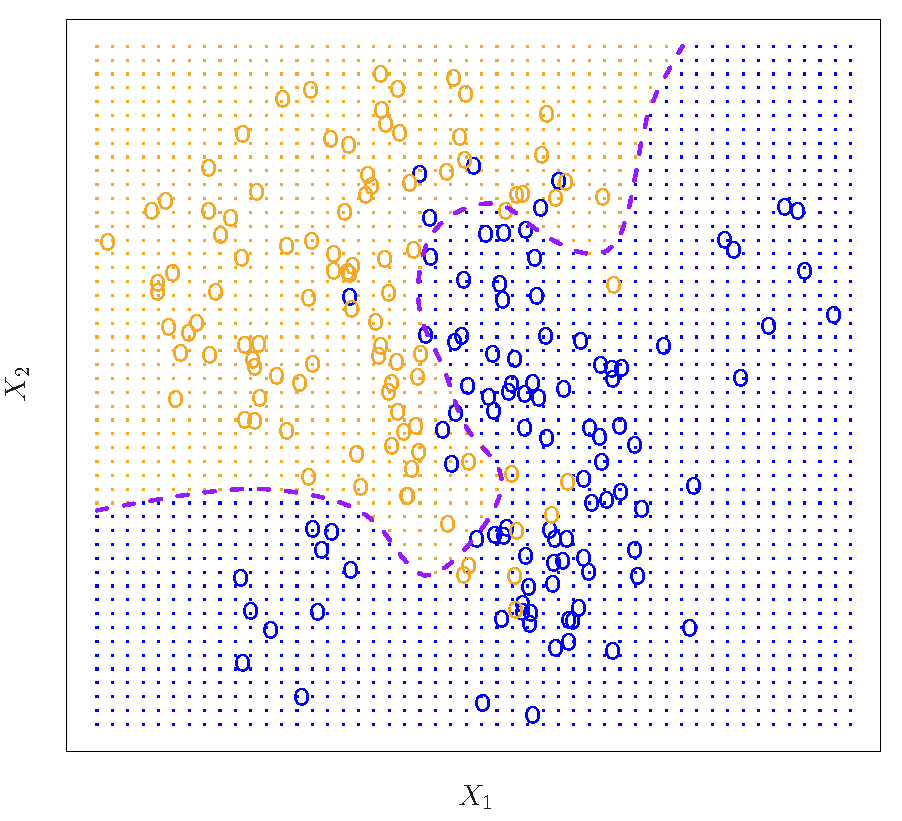
\includegraphics[width=1\textwidth,height=12.5in]{2.13.pdf}
\caption{Alt}
\end{figure}

Or like this graph also brazenly borrowed from Gareth James?

\begin{figure}
\centering
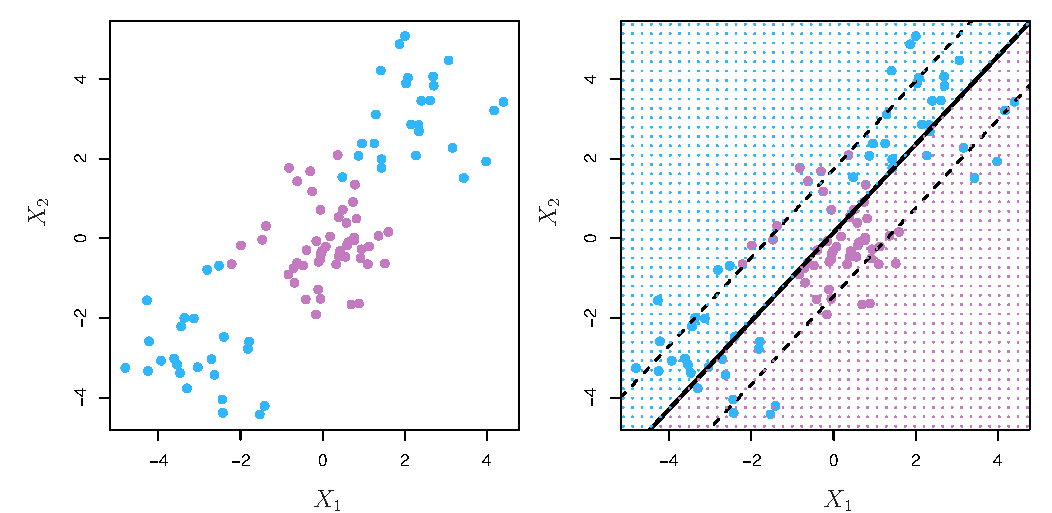
\includegraphics[width=1\textwidth,height=12.5in]{9.8.pdf}
\caption{Alt}
\end{figure}

The K-nearest neighbor approach will help with the first predicament.

But for the second predicament we are going to need something different.

And now for something different\ldots{}

Suppose that we have data that look like thus:

\begin{figure}
\centering
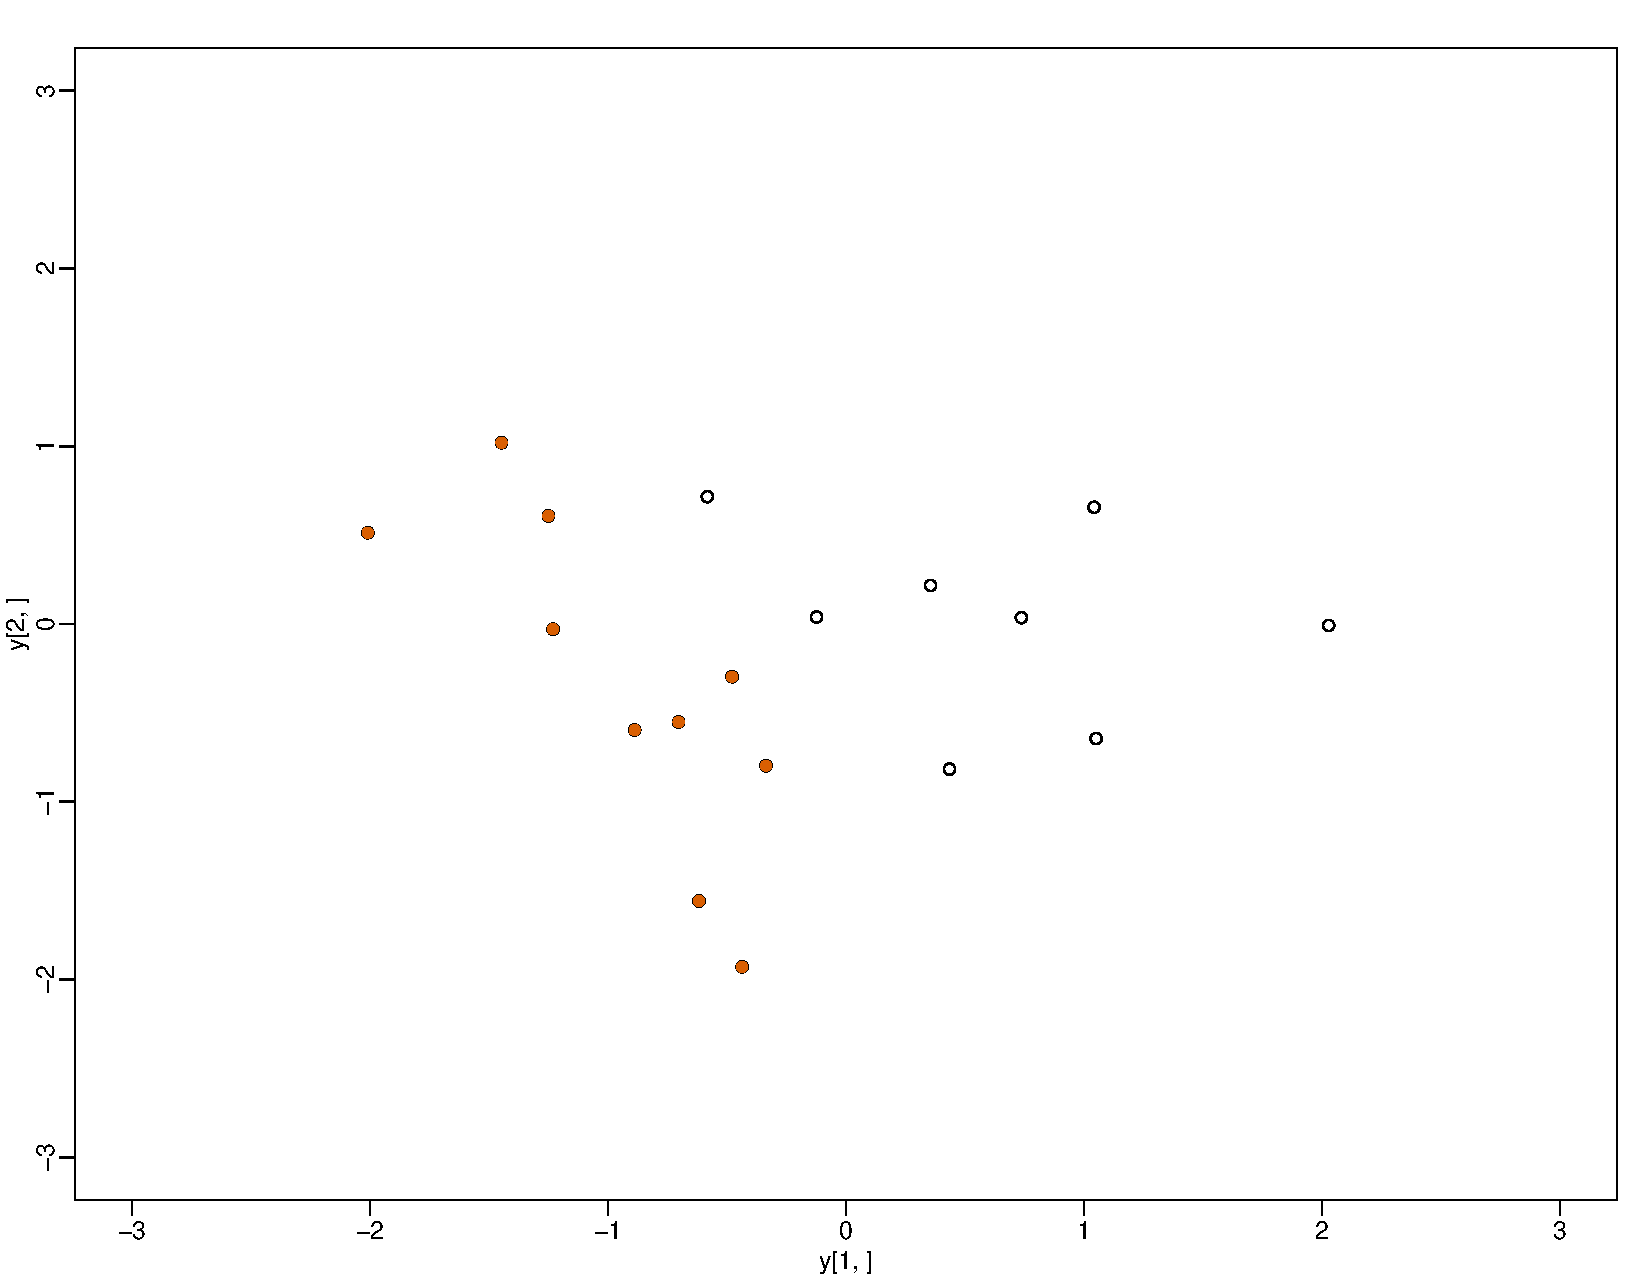
\includegraphics[width=1\textwidth,height=12.5in]{MMCpointsonly.pdf}
\caption{Alt}
\end{figure}

These data can be perfectly separated by a hyperplane (in 2-dimensions,
this is a line), like so:

\begin{figure}
\centering
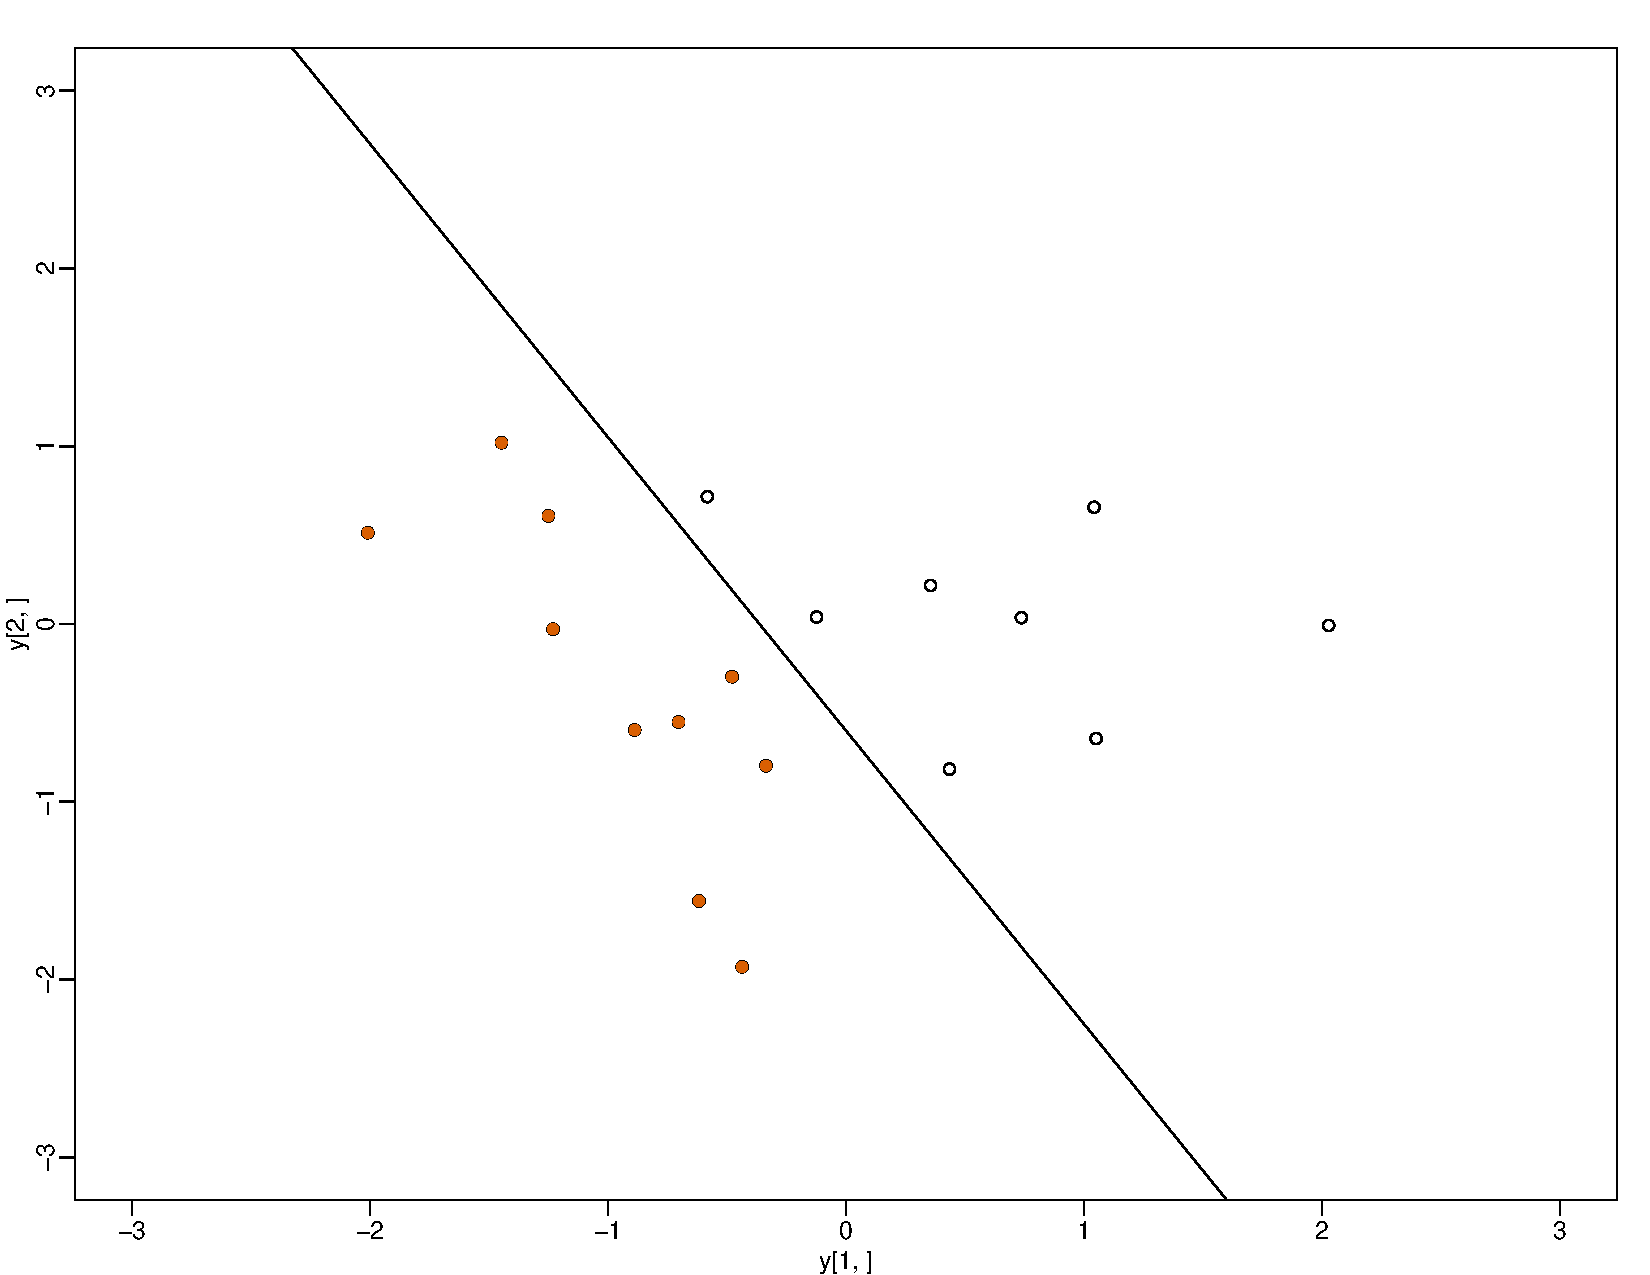
\includegraphics[width=1\textwidth,height=12.5in]{MMChyperplane.pdf}
\caption{Alt}
\end{figure}

This line is the one that is the furthest from the closest points of
either group, and it is called the Maximal Margin Classifier, that is,
the margins to the closest points are as large as possible for any line
that you could draw, as so:

\begin{figure}
\centering
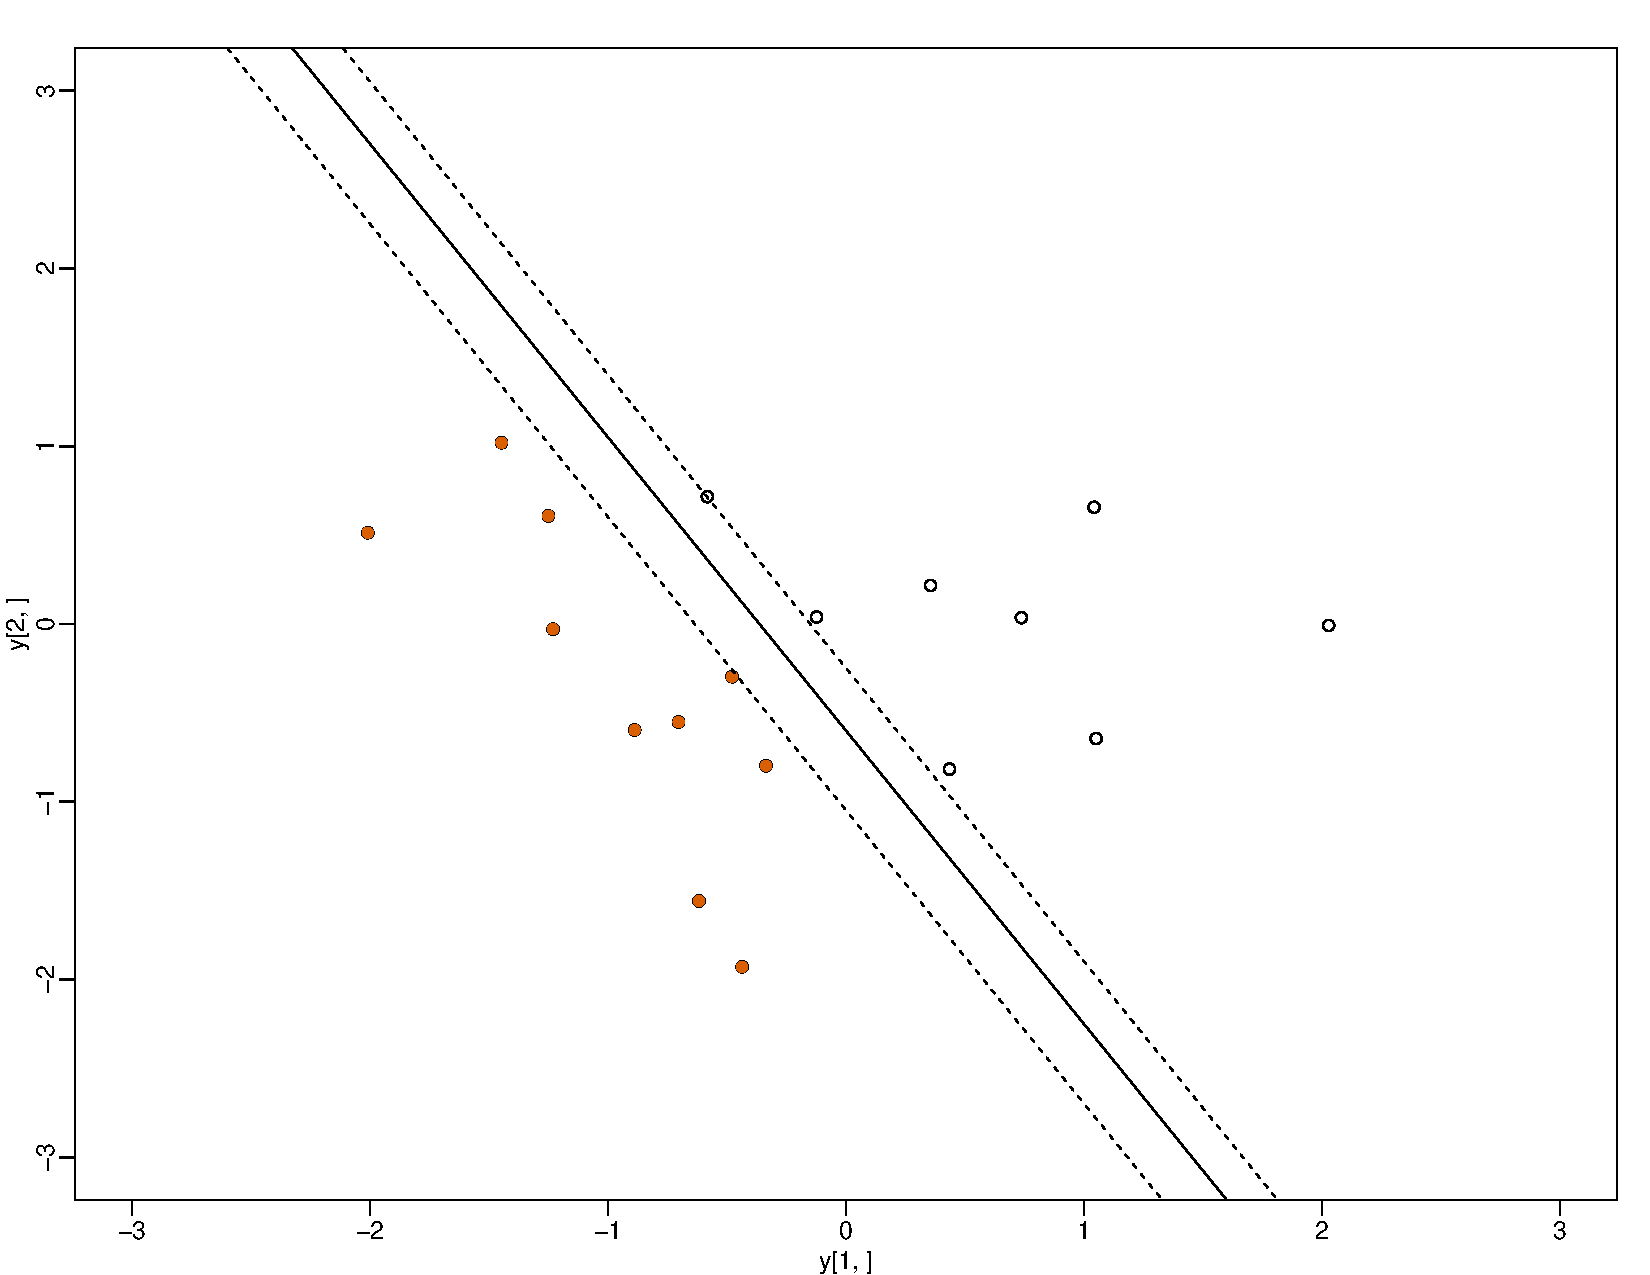
\includegraphics[width=1\textwidth,height=12.5in]{MMCdash.pdf}
\caption{Alt}
\end{figure}

This classifier will only work if you can draw a hyperplane to separate
the groups.

The problem with MMC's - they are very sensitive to the tiny changes in
the data. For instance, look at the figure below. There is only 1 point
that is different from the previous scatterplot.

\begin{figure}
\centering
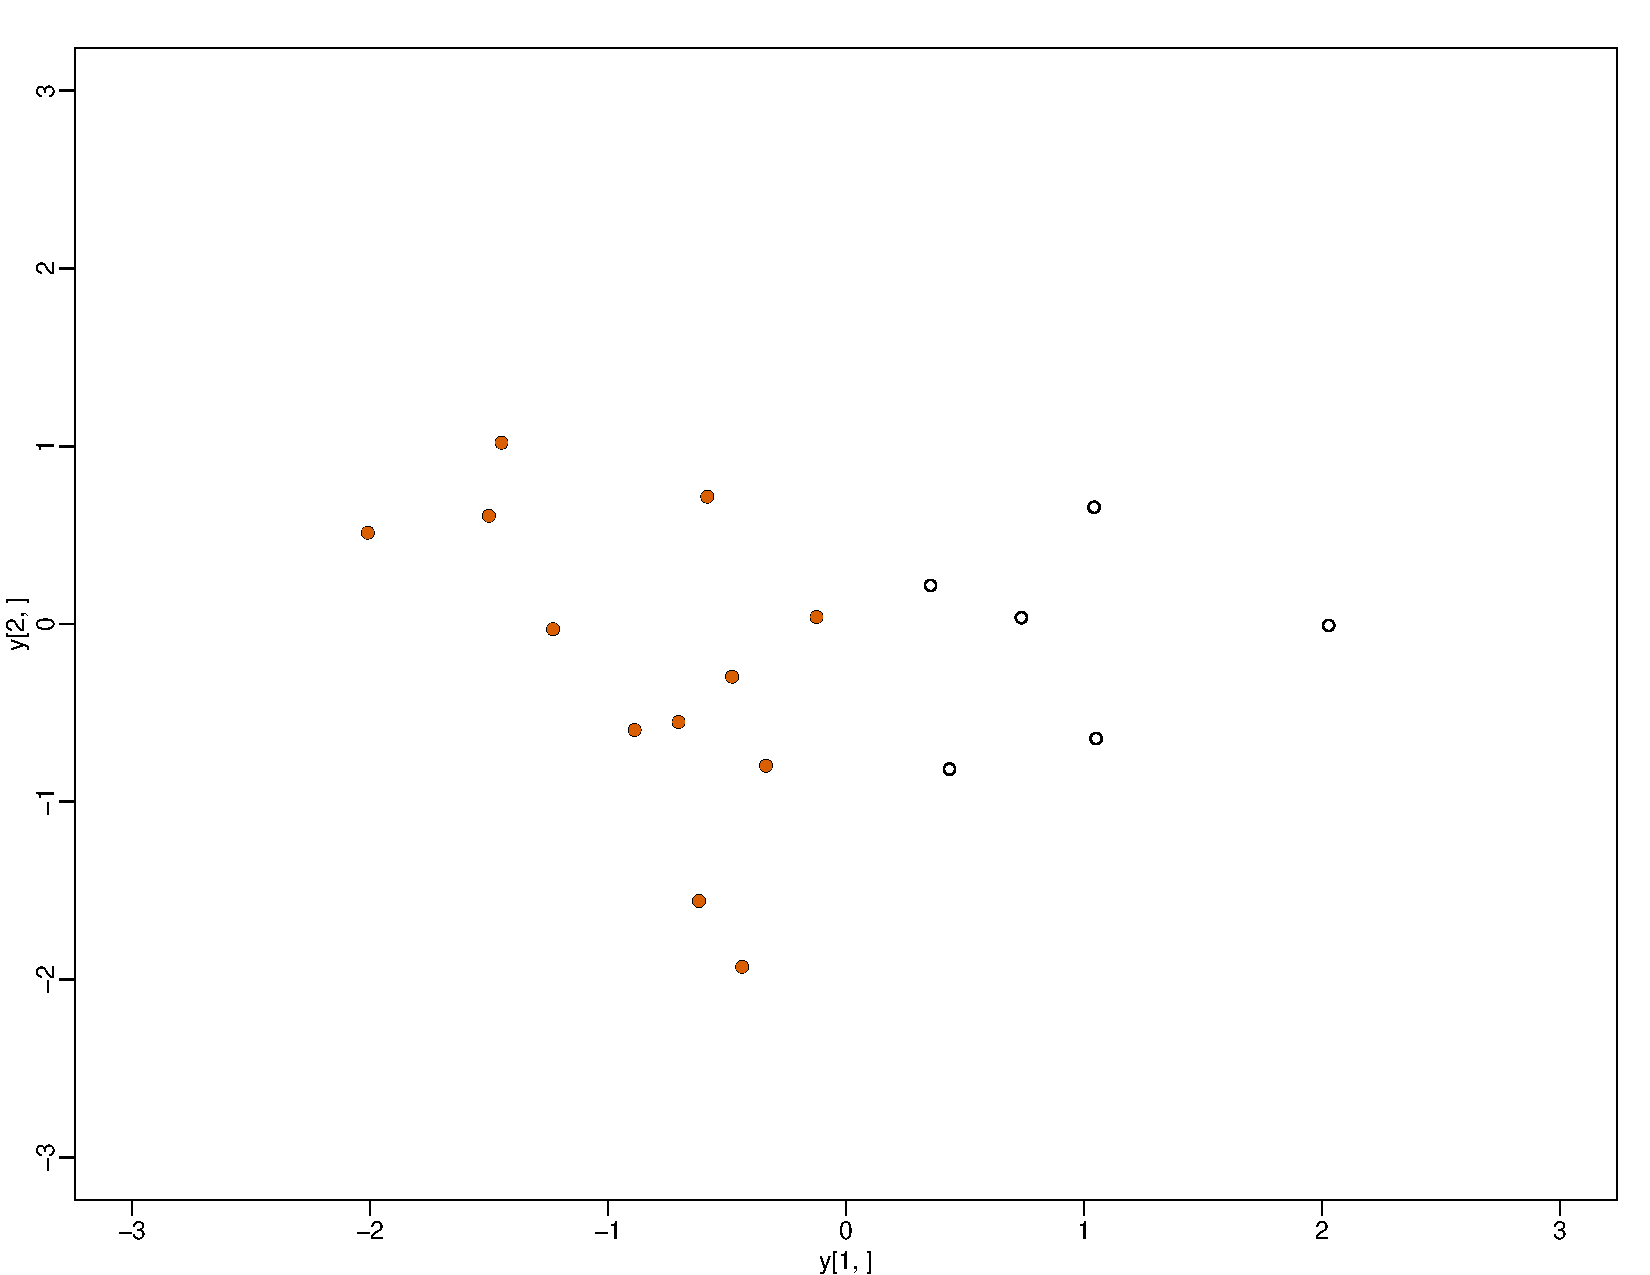
\includegraphics[width=1\textwidth,height=12.5in]{MMConepointmore.pdf}
\caption{Alt}
\end{figure}

Yet, that causes a huge change in the MMC, as shown below:

\begin{figure}
\centering
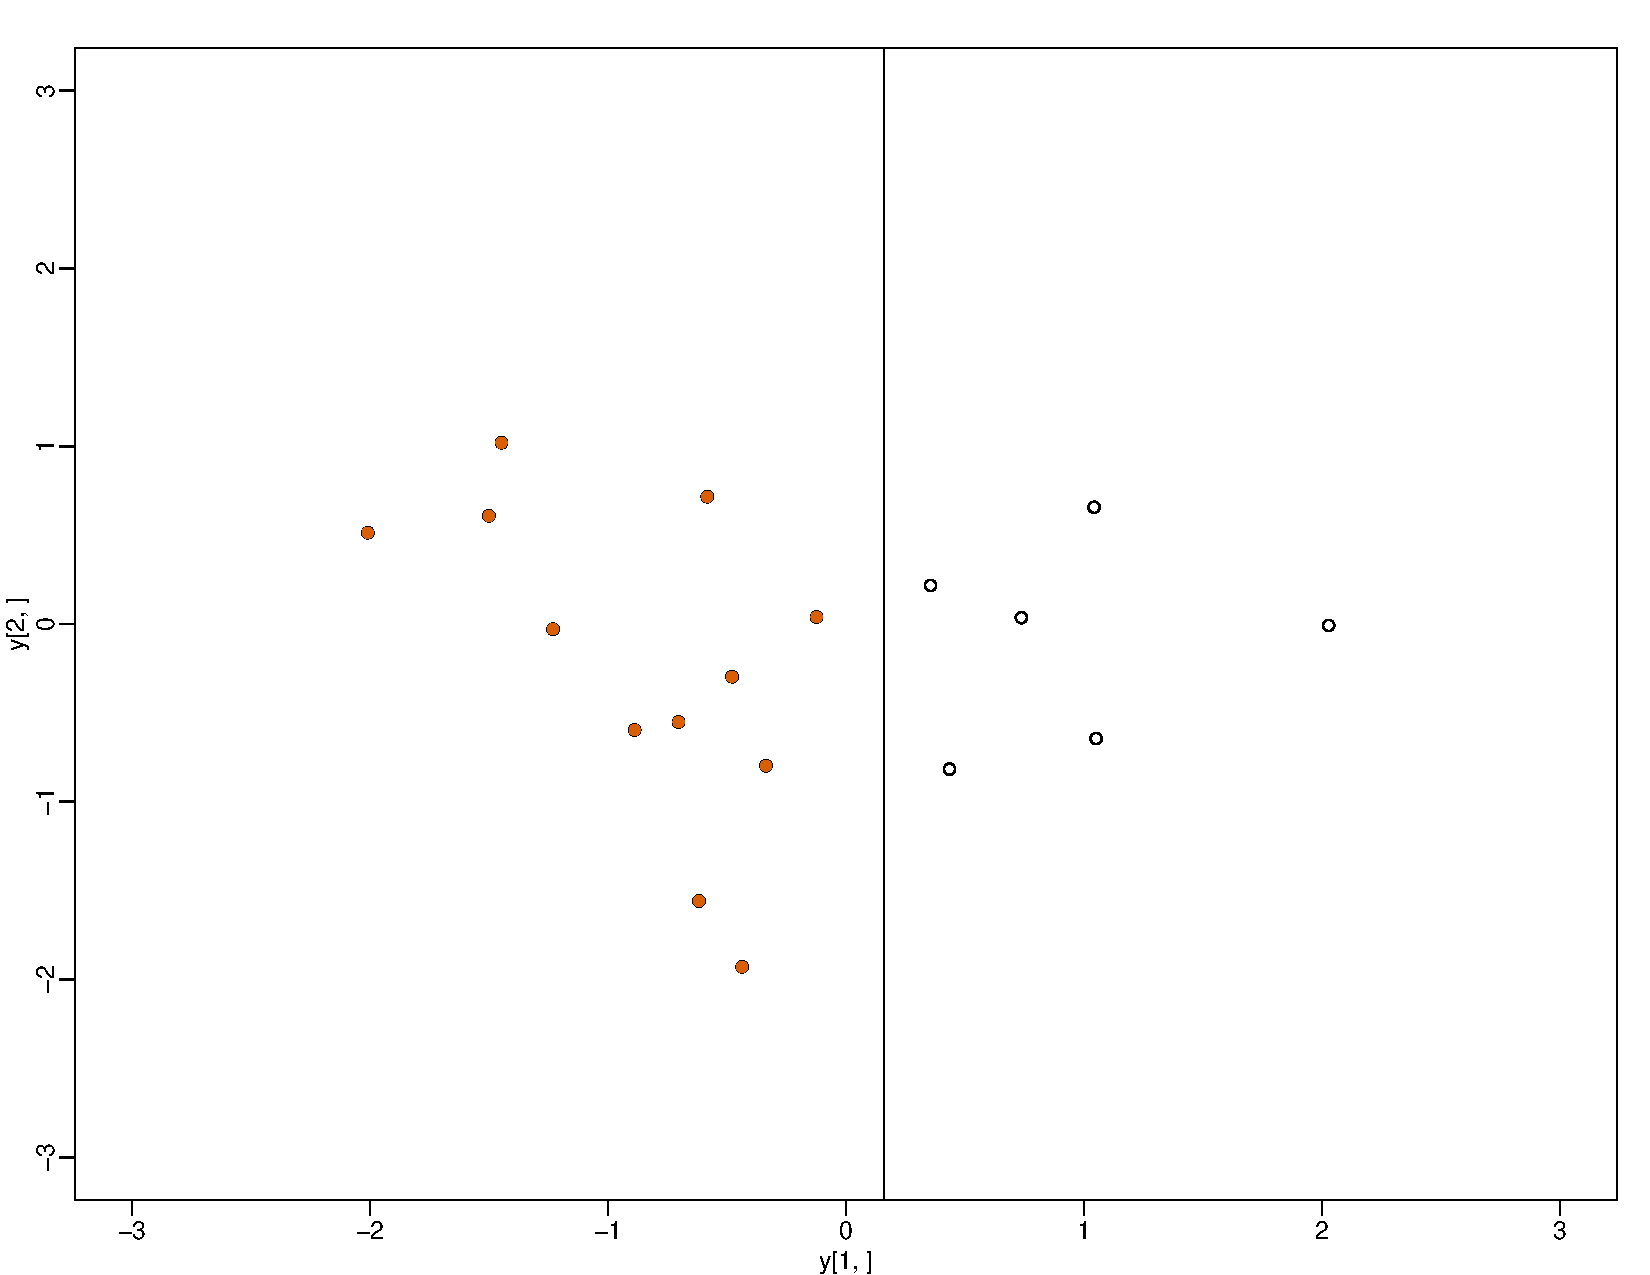
\includegraphics[width=1\textwidth,height=12.5in]{MMConepointorehyperplane.pdf}
\caption{Alt}
\end{figure}

What if your data look like this:

\begin{figure}
\centering
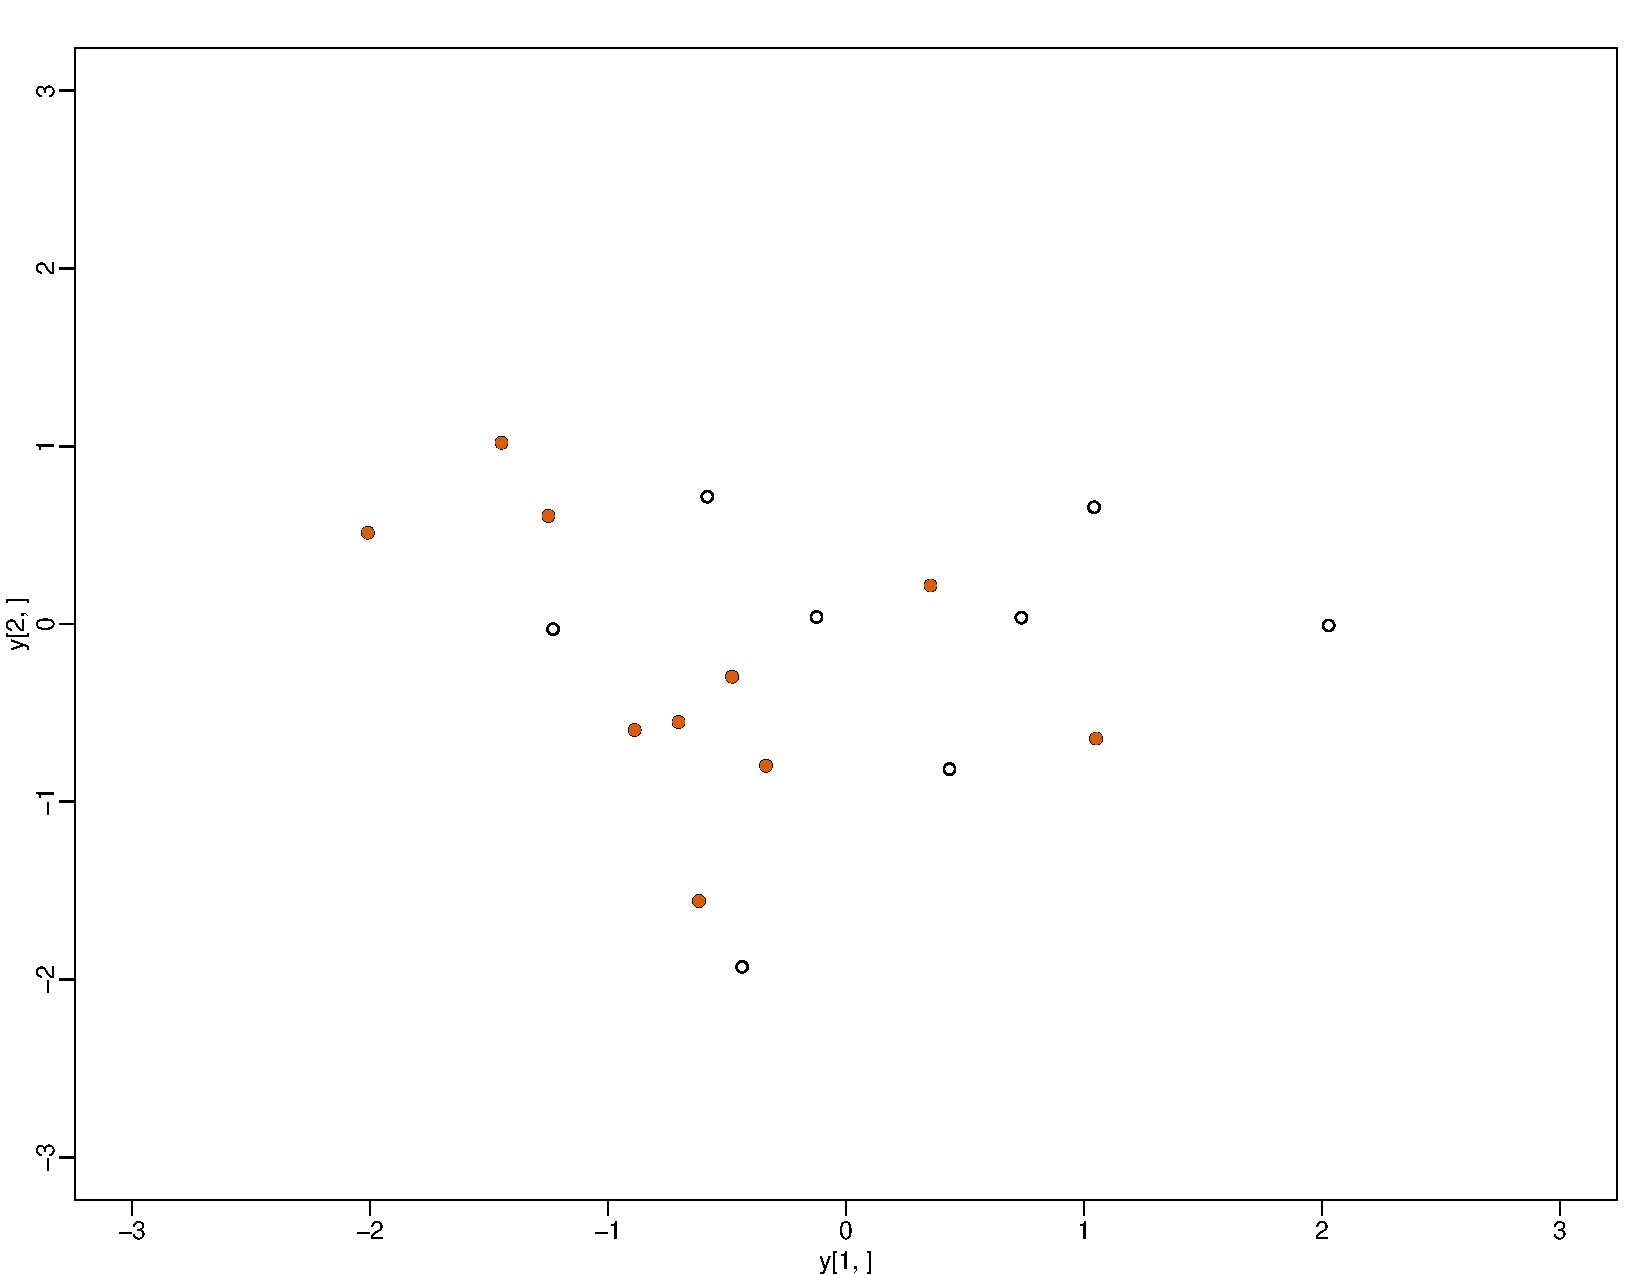
\includegraphics[width=1\textwidth,height=12.5in]{MMCnogo.pdf}
\caption{Alt}
\end{figure}

For these data you can't draw a line that separates them.

What to do?

\hypertarget{support-vector-classifiers}{%
\subsubsection{Support Vector
Classifiers}\label{support-vector-classifiers}}

The goal is to create a classifier created based on a hyperplane that
may not perfectly separate classes but does offer greater robustness to
the effects of individual observations, and better classification of
most of the training observations. The \emph{support vector classifier}
does exactly that. This is sometimes called a \emph{soft margin
classifier}

Recall our MMC. It could be that a classifier like this might actually
work - it classifies 5 wrong, but gets most right, and it should be
fairly robust. The support vectors in this case are the dashed lines.
The objective is to minimize prediction error, but we can allow some
values to be on the incorrect side of the margin or even the incorrect
side of the hyperplane. In that case the margins are considered
``soft''.

\hypertarget{support-vector-machines}{%
\subsubsection{Support Vector Machines}\label{support-vector-machines}}

All of that is fine and good, but what if we have data that look as
follows (brazenly borrowed by Gareth James):

\begin{figure}
\centering
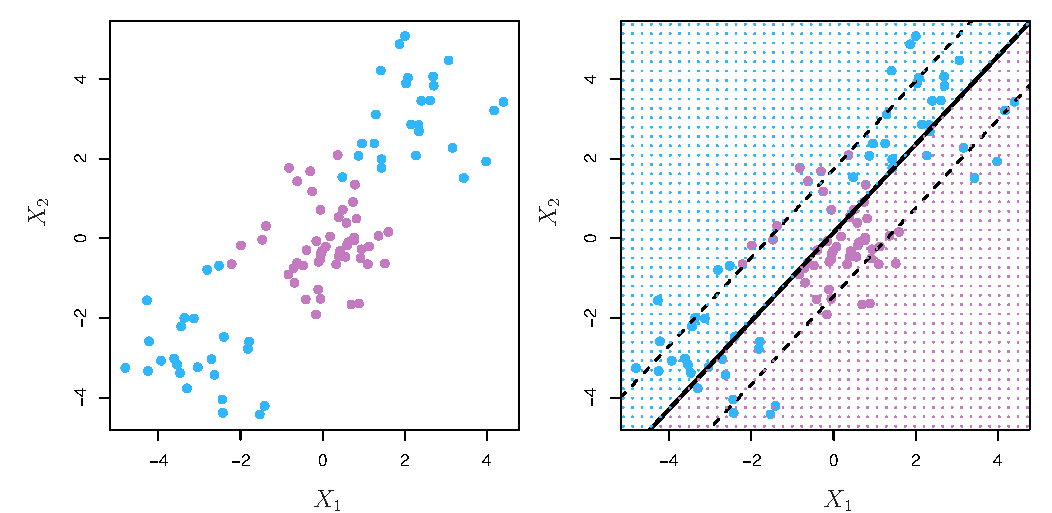
\includegraphics[width=1\textwidth,height=12.5in]{9.8.pdf}
\caption{Alt}
\end{figure}

As we see on the left there appear to be at least 2, maybe 3 groups.
And, as we see on the right, an SVC is useless.

So we have to think about using \emph{non-linear} boundaries instead, as
shown below (brazenly borrowed by Gareth James):

\begin{figure}
\centering
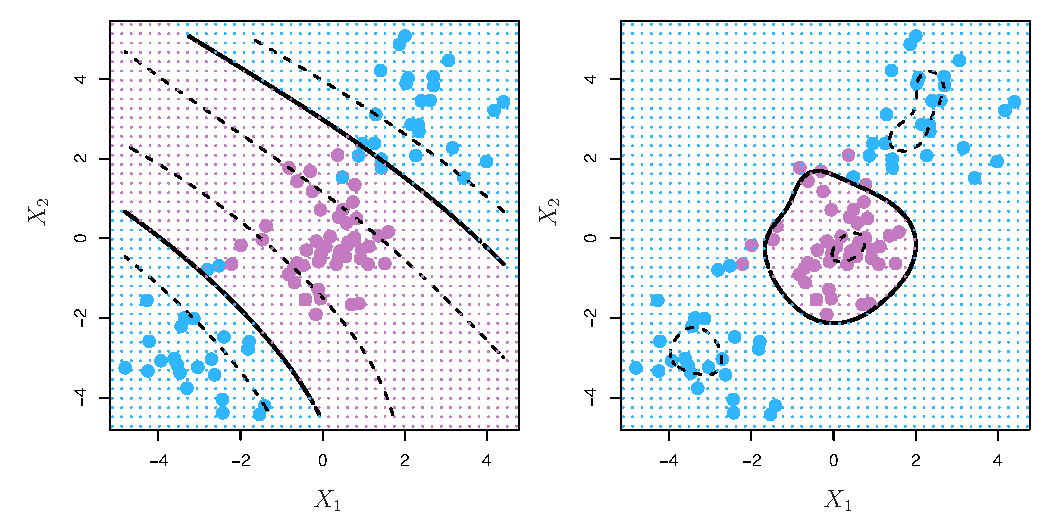
\includegraphics[width=1\textwidth,height=12.5in]{9.9.pdf}
\caption{Alt}
\end{figure}

So we will want to \emph{enlarge} our feature space by using functions
of our features, in particular, polynomial terms, in order to develop
these boundaries. We will do this by using what is called a
\emph{kernel} function. The definition of a kernel is beyond the scope
of this class. But it turns out that there are computational methods to
produce these extended features in a computationally efficient manner,
and that the linear SVC can be represented by these features as well.
All of this will only involve what is called the inner product of two
observations. For two observations X\_i and X\_\{i'\} the inner product
is

\begin{equation}

<X_i, X_{i'}> = \sum_{j=1}^{p} {x_{ij}x_{i'j}}

\end{equation}

Let's look at an example or two. Consider the Khan dataset in the ISLR
package. It contains expression levels for a number of genes
corresponding to four types of small round blue cell tumors. There is a
set of training data and a set of testing data.

\begin{Shaded}
\begin{Highlighting}[]
\CommentTok{\# Call up ISLR, which contains the dataset, and e1071, which contains the function for fitting an SVM}

\FunctionTok{library}\NormalTok{(ISLR)}
\FunctionTok{library}\NormalTok{(e1071)}

\CommentTok{\# What is in the Khan data set?}

\FunctionTok{names}\NormalTok{(Khan)}
\end{Highlighting}
\end{Shaded}

\begin{verbatim}
## [1] "xtrain" "xtest"  "ytrain" "ytest"
\end{verbatim}

\begin{Shaded}
\begin{Highlighting}[]
\CommentTok{\# What are the dimensions of the objects in the Khan dataset?}

\FunctionTok{dim}\NormalTok{(Khan}\SpecialCharTok{$}\NormalTok{xtrain)}
\end{Highlighting}
\end{Shaded}

\begin{verbatim}
## [1]   63 2308
\end{verbatim}

\begin{Shaded}
\begin{Highlighting}[]
\FunctionTok{dim}\NormalTok{(Khan}\SpecialCharTok{$}\NormalTok{xtest)}
\end{Highlighting}
\end{Shaded}

\begin{verbatim}
## [1]   20 2308
\end{verbatim}

\begin{Shaded}
\begin{Highlighting}[]
\FunctionTok{dim}\NormalTok{(Khan}\SpecialCharTok{$}\NormalTok{ytrain)}
\end{Highlighting}
\end{Shaded}

\begin{verbatim}
## NULL
\end{verbatim}

\begin{Shaded}
\begin{Highlighting}[]
\FunctionTok{dim}\NormalTok{(Khan}\SpecialCharTok{$}\NormalTok{ytest)}
\end{Highlighting}
\end{Shaded}

\begin{verbatim}
## NULL
\end{verbatim}

\begin{Shaded}
\begin{Highlighting}[]
\CommentTok{\# How do the observations in the training and testing datasets distribute among the tumor type classes?}

\FunctionTok{table}\NormalTok{(Khan}\SpecialCharTok{$}\NormalTok{ytrain)}
\end{Highlighting}
\end{Shaded}

\begin{verbatim}
## 
##  1  2  3  4 
##  8 23 12 20
\end{verbatim}

\begin{Shaded}
\begin{Highlighting}[]
\FunctionTok{table}\NormalTok{(Khan}\SpecialCharTok{$}\NormalTok{ytest)}
\end{Highlighting}
\end{Shaded}

\begin{verbatim}
## 
## 1 2 3 4 
## 3 6 6 5
\end{verbatim}

We will use a support vector approach to predict tumor type from gene
expression levels.

There are a very large number of features relative to the number of
observations. In this case, we should use a linear kernel.

\begin{Shaded}
\begin{Highlighting}[]
\CommentTok{\# Create the data frame consisting of the training data}

\NormalTok{dat }\OtherTok{\textless{}{-}} \FunctionTok{data.frame}\NormalTok{(}\AttributeTok{x=}\NormalTok{Khan}\SpecialCharTok{$}\NormalTok{xtrain, }\AttributeTok{y =} \FunctionTok{as.factor}\NormalTok{(Khan}\SpecialCharTok{$}\NormalTok{ytrain))}

\CommentTok{\# Run the svm() function on the training data using a linear kernel}

\NormalTok{out }\OtherTok{\textless{}{-}} \FunctionTok{svm}\NormalTok{(y}\SpecialCharTok{\textasciitilde{}}\NormalTok{., }\AttributeTok{data =}\NormalTok{ dat, }\AttributeTok{kernel =} \StringTok{"linear"}\NormalTok{)}

\CommentTok{\# What is in this new object created by the svm() function?}

\FunctionTok{summary}\NormalTok{(out)}
\end{Highlighting}
\end{Shaded}

\begin{verbatim}
## 
## Call:
## svm(formula = y ~ ., data = dat, kernel = "linear")
## 
## 
## Parameters:
##    SVM-Type:  C-classification 
##  SVM-Kernel:  linear 
##        cost:  1 
## 
## Number of Support Vectors:  58
## 
##  ( 20 20 11 7 )
## 
## 
## Number of Classes:  4 
## 
## Levels: 
##  1 2 3 4
\end{verbatim}

\begin{Shaded}
\begin{Highlighting}[]
\CommentTok{\# How well does this SVM predict the training data?}

\FunctionTok{table}\NormalTok{(out}\SpecialCharTok{$}\NormalTok{fitted, dat}\SpecialCharTok{$}\NormalTok{y)}
\end{Highlighting}
\end{Shaded}

\begin{verbatim}
##    
##      1  2  3  4
##   1  8  0  0  0
##   2  0 23  0  0
##   3  0  0 12  0
##   4  0  0  0 20
\end{verbatim}

We see that there are no training errors. This is not surprising, since
the large number of features relative to observations guarantees that
you can find any number of hyperplanes that will fully separate the
observations.

So what about the SVM's performance on the test observations?

\begin{Shaded}
\begin{Highlighting}[]
\CommentTok{\# Create the dataframe for the testing data}

\NormalTok{dat.test }\OtherTok{\textless{}{-}} \FunctionTok{data.frame}\NormalTok{(}\AttributeTok{x=}\NormalTok{Khan}\SpecialCharTok{$}\NormalTok{xtest, }\AttributeTok{y=} \FunctionTok{as.factor}\NormalTok{(Khan}\SpecialCharTok{$}\NormalTok{ytest))}

\CommentTok{\# Use the SVM we just created to classify the test dataset}

\NormalTok{pred.test }\OtherTok{\textless{}{-}} \FunctionTok{predict}\NormalTok{(out, }\AttributeTok{newdata =}\NormalTok{ dat.test)}

\CommentTok{\# How well does this SVM do at classifying the test dataset?}

\FunctionTok{table}\NormalTok{(pred.test, dat.test}\SpecialCharTok{$}\NormalTok{y)}
\end{Highlighting}
\end{Shaded}

\begin{verbatim}
##          
## pred.test 1 2 3 4
##         1 3 0 0 0
##         2 0 6 2 0
##         3 0 0 4 0
##         4 0 0 0 5
\end{verbatim}

We see that there are 2 errors, or a 10\% error rate.

\hypertarget{unsupervised-learning}{%
\section{Unsupervised learning}\label{unsupervised-learning}}

For Act III today we will talk about unsupervised learning - that is we
want to discover patterns in the data without an \emph{a priori}
understanding of any grouping structure.

There are a couple of ways to do this. We will talk about k-means
clustering and principal components analysis (PCA).

\hypertarget{clustering}{%
\subsection{Clustering}\label{clustering}}

You have probably all seen an example of an evolutionary tree -
sometimes also called a dendogram. Although biologists will imagine that
at each branching point there was an actual being (plant or animal), the
descendants of whom split into groups that evolved in different
directions. They will group similar beings close to each other, and
not-so-similar ones at further distances. But you will note that there
is no outcome variable - just decisions as to what is close and what is
far with respect to relatedness.

In general you can use trees to describe the similarity between objects,
regardless of how they came to be. The tree may or may not be a
reflection of something deeper about the objects and their relationships
- it can just be a simple way to visualize relationships.

To develop these trees from a set of numerical variables, none of which
constitutes a \emph{response} you would need to plot the data as points
in space then make branches based on how close together points are. This
technique is called \emph{hierarchical clustering}.

The \texttt{NCI60} dataset contains microarray gene expression levels on
6830 genes for 68 cancer cell lines. Although cancer cell type is
recorded, we are going to explore how the data group without considering
this variable, then look at how closely the \emph{de novo} grouping
compares to the cell types. The data come from the publication by Ross
et al (Nature Genetics, 2000). The dataset is available in the
\texttt{ISLR} package. The \texttt{ape} package contains many functions
for phylogenetic trees.

\begin{Shaded}
\begin{Highlighting}[]
\FunctionTok{library}\NormalTok{(tidyverse)}
\FunctionTok{library}\NormalTok{(maps)}
\FunctionTok{library}\NormalTok{(ISLR)}
\FunctionTok{library}\NormalTok{(ape)}

\NormalTok{nci.labs }\OtherTok{\textless{}{-}}\NormalTok{ NCI60}\SpecialCharTok{$}\NormalTok{labs }\CommentTok{\# Labels for checking later}
\NormalTok{nci.data }\OtherTok{\textless{}{-}}\NormalTok{ NCI60}\SpecialCharTok{$}\NormalTok{data}

\CommentTok{\# What do the data look like?}
\FunctionTok{dim}\NormalTok{(nci.data)}
\end{Highlighting}
\end{Shaded}

\begin{verbatim}
## [1]   64 6830
\end{verbatim}

\begin{Shaded}
\begin{Highlighting}[]
\FunctionTok{length}\NormalTok{(nci.labs)}
\end{Highlighting}
\end{Shaded}

\begin{verbatim}
## [1] 64
\end{verbatim}

\begin{Shaded}
\begin{Highlighting}[]
\NormalTok{nci.labs[}\DecValTok{1}\SpecialCharTok{:}\DecValTok{4}\NormalTok{]}
\end{Highlighting}
\end{Shaded}

\begin{verbatim}
## [1] "CNS"   "CNS"   "CNS"   "RENAL"
\end{verbatim}

\begin{Shaded}
\begin{Highlighting}[]
\FunctionTok{table}\NormalTok{(nci.labs)}
\end{Highlighting}
\end{Shaded}

\begin{verbatim}
## nci.labs
##      BREAST         CNS       COLON K562A-repro K562B-repro    LEUKEMIA 
##           7           5           7           1           1           6 
## MCF7A-repro MCF7D-repro    MELANOMA       NSCLC     OVARIAN    PROSTATE 
##           1           1           8           9           6           2 
##       RENAL     UNKNOWN 
##           9           1
\end{verbatim}

\begin{Shaded}
\begin{Highlighting}[]
\CommentTok{\# Scale the data before clustering}
\NormalTok{sd.data }\OtherTok{\textless{}{-}} \FunctionTok{scale}\NormalTok{(nci.data)}

\CommentTok{\# Calculate Euclidean distance between each pair of points}
\NormalTok{data.dist }\OtherTok{\textless{}{-}} \FunctionTok{dist}\NormalTok{(sd.data)}

\CommentTok{\# Plot the tree, default linkage is \textquotesingle{}complete\textquotesingle{}}
\FunctionTok{plot}\NormalTok{(}
  \FunctionTok{hclust}\NormalTok{(data.dist),}
  \AttributeTok{labels =}\NormalTok{ nci.labs,}
  \AttributeTok{main =} \StringTok{"Complete Linkage"}\NormalTok{,}
  \AttributeTok{xlab =} \StringTok{""}\NormalTok{,}
  \AttributeTok{sub =} \StringTok{""}\NormalTok{,}
  \AttributeTok{ylab =} \StringTok{""}
\NormalTok{)}
\end{Highlighting}
\end{Shaded}

\includegraphics{ML_part2_2021_files/figure-latex/unnamed-chunk-12-1.pdf}

\begin{Shaded}
\begin{Highlighting}[]
\CommentTok{\# Plot the tree, linkage is \textquotesingle{}average\textquotesingle{}}
\FunctionTok{plot}\NormalTok{(}
  \FunctionTok{hclust}\NormalTok{(data.dist),}
  \AttributeTok{method =} \StringTok{"average"}\NormalTok{,}
  \AttributeTok{labels =}\NormalTok{ nci.labs,}
  \AttributeTok{main =} \StringTok{"Average Linkage"}\NormalTok{,}
  \AttributeTok{xlab =} \StringTok{""}\NormalTok{,}
  \AttributeTok{sub =} \StringTok{""}\NormalTok{,}
  \AttributeTok{ylab =} \StringTok{""}
\NormalTok{)}
\end{Highlighting}
\end{Shaded}

\includegraphics{ML_part2_2021_files/figure-latex/unnamed-chunk-12-2.pdf}

\begin{Shaded}
\begin{Highlighting}[]
\CommentTok{\# Plot the tree, default linkage is \textquotesingle{}single\textquotesingle{}}
\FunctionTok{plot}\NormalTok{(}
  \FunctionTok{hclust}\NormalTok{(data.dist),}
  \AttributeTok{method =} \StringTok{"single"}\NormalTok{,}
  \AttributeTok{labels =}\NormalTok{ nci.labs,}
  \AttributeTok{main =} \StringTok{"Single Linkage"}\NormalTok{,}
  \AttributeTok{xlab =} \StringTok{""}\NormalTok{,}
  \AttributeTok{sub =} \StringTok{""}\NormalTok{,}
  \AttributeTok{ylab =} \StringTok{""}
\NormalTok{)}
\end{Highlighting}
\end{Shaded}

\includegraphics{ML_part2_2021_files/figure-latex/unnamed-chunk-12-3.pdf}

How do you think these trees compare?

Which one should we use?

\begin{Shaded}
\begin{Highlighting}[]
\CommentTok{\# Let\textquotesingle{}s use complete linkage and cut into 4 clusters}

\NormalTok{hc.out }\OtherTok{\textless{}{-}} \FunctionTok{hclust}\NormalTok{(}\FunctionTok{dist}\NormalTok{(sd.data))}
\NormalTok{hc.clusters }\OtherTok{\textless{}{-}} \FunctionTok{cutree}\NormalTok{(hc.out, }\DecValTok{4}\NormalTok{)}
\FunctionTok{table}\NormalTok{(hc.clusters, nci.labs)}
\end{Highlighting}
\end{Shaded}

\begin{verbatim}
##            nci.labs
## hc.clusters BREAST CNS COLON K562A-repro K562B-repro LEUKEMIA MCF7A-repro
##           1      2   3     2           0           0        0           0
##           2      3   2     0           0           0        0           0
##           3      0   0     0           1           1        6           0
##           4      2   0     5           0           0        0           1
##            nci.labs
## hc.clusters MCF7D-repro MELANOMA NSCLC OVARIAN PROSTATE RENAL UNKNOWN
##           1           0        8     8       6        2     8       1
##           2           0        0     1       0        0     1       0
##           3           0        0     0       0        0     0       0
##           4           1        0     0       0        0     0       0
\end{verbatim}

Where are the leukemia cases? What about the breast cancer cases?

Where in the tree is the cut that yielded the 4 clusters?

\begin{Shaded}
\begin{Highlighting}[]
\CommentTok{\# plot the cut in the tree that yielded the 4 clusters}

\FunctionTok{plot}\NormalTok{(hc.out, }\AttributeTok{labels =}\NormalTok{ nci.labs)}
\FunctionTok{abline}\NormalTok{(}\AttributeTok{h=}\DecValTok{139}\NormalTok{, }\AttributeTok{col =} \StringTok{"red"}\NormalTok{)}
\end{Highlighting}
\end{Shaded}

\includegraphics{ML_part2_2021_files/figure-latex/unnamed-chunk-14-1.pdf}

Let's look at the summary of the tree:

\begin{Shaded}
\begin{Highlighting}[]
\CommentTok{\# Summary of hierarchical clustering}
\NormalTok{hc.out}
\end{Highlighting}
\end{Shaded}

\begin{verbatim}
## 
## Call:
## hclust(d = dist(sd.data))
## 
## Cluster method   : complete 
## Distance         : euclidean 
## Number of objects: 64
\end{verbatim}

\hypertarget{k-means-clustering}{%
\subsubsection{K-means clustering}\label{k-means-clustering}}

An alternative method of clustering is \emph{K-means clustering}. Again,
we place our points in space, and decide on groups, but we do so without
consideration of hierarchy.

Let's see how these two types of clustering compare on the
\texttt{NCI60} dataset:

\begin{Shaded}
\begin{Highlighting}[]
\CommentTok{\# K{-}means clustering with K=4 (from the hierarchical clustering number)}

\FunctionTok{set.seed}\NormalTok{(}\DecValTok{40523}\NormalTok{)}
\NormalTok{km.out }\OtherTok{=} \FunctionTok{kmeans}\NormalTok{(sd.data, }\DecValTok{4}\NormalTok{, }\AttributeTok{nstart =} \DecValTok{20}\NormalTok{)}
\NormalTok{km.clusters }\OtherTok{=}\NormalTok{ km.out}\SpecialCharTok{$}\NormalTok{cluster}
\FunctionTok{table}\NormalTok{(km.clusters, hc.clusters)}
\end{Highlighting}
\end{Shaded}

\begin{verbatim}
##            hc.clusters
## km.clusters  1  2  3  4
##           1  9  0  0  0
##           2 11  0  0  9
##           3 20  7  0  0
##           4  0  0  8  0
\end{verbatim}

How do the clustering methods compare?

Which clusters are found by both methods?

\hypertarget{another-example}{%
\subsubsection{Another example}\label{another-example}}

Let's look at another example. We have data about the cities in the
world in the dataset\texttt{WorldCities}. For the 4000 largest cities,
considering \emph{only} latitude and longitude (two of the
\emph{features} of this dataset), how would these data items group and
plot?

\begin{Shaded}
\begin{Highlighting}[]
\CommentTok{\#get the 4000 largest cities, variables are only latitude and longitude}

\NormalTok{BigCities }\OtherTok{\textless{}{-}}\NormalTok{ world.cities }\SpecialCharTok{\%\textgreater{}\%}
  \FunctionTok{arrange}\NormalTok{(}\FunctionTok{desc}\NormalTok{(pop)) }\SpecialCharTok{\%\textgreater{}\%}
  \FunctionTok{head}\NormalTok{(}\DecValTok{4000}\NormalTok{) }\SpecialCharTok{\%\textgreater{}\%}
\NormalTok{  dplyr}\SpecialCharTok{::}\FunctionTok{select}\NormalTok{(long, lat)}
\FunctionTok{glimpse}\NormalTok{(BigCities)}
\end{Highlighting}
\end{Shaded}

\begin{verbatim}
## Rows: 4,000
## Columns: 2
## $ long <dbl> 121.47, 72.82, 67.01, -58.37, 77.21, 120.97, 37.62, 126.99, -46.6~
## $ lat  <dbl> 31.23, 18.96, 24.86, -34.61, 28.67, 14.62, 55.75, 37.56, -23.53, ~
\end{verbatim}

Notice that the \texttt{BigCities} dataset does not even contain the
names of the cities, \emph{just} latitude and longitude.

\begin{Shaded}
\begin{Highlighting}[]
\FunctionTok{library}\NormalTok{(mclust)}
\FunctionTok{set.seed}\NormalTok{(}\DecValTok{15}\NormalTok{)}
\NormalTok{city\_clusts }\OtherTok{\textless{}{-}}\NormalTok{ BigCities }\SpecialCharTok{\%\textgreater{}\%}
  \FunctionTok{kmeans}\NormalTok{(}\AttributeTok{centers =} \DecValTok{6}\NormalTok{) }\SpecialCharTok{\%\textgreater{}\%}
  \FunctionTok{fitted}\NormalTok{(}\StringTok{"classes"}\NormalTok{) }\SpecialCharTok{\%\textgreater{}\%}
  \FunctionTok{as.character}\NormalTok{()}
\NormalTok{BigCities }\OtherTok{\textless{}{-}}\NormalTok{ BigCities }\SpecialCharTok{\%\textgreater{}\%} \FunctionTok{mutate}\NormalTok{(}\AttributeTok{cluster =}\NormalTok{ city\_clusts)}
\NormalTok{BigCities }\SpecialCharTok{\%\textgreater{}\%} \FunctionTok{ggplot}\NormalTok{(}\FunctionTok{aes}\NormalTok{(}\AttributeTok{x=}\NormalTok{long, }\AttributeTok{y=}\NormalTok{lat)) }\SpecialCharTok{+}
  \FunctionTok{geom\_point}\NormalTok{(}\FunctionTok{aes}\NormalTok{(}\AttributeTok{color =}\NormalTok{ cluster), }\AttributeTok{alpha =} \FloatTok{0.5}\NormalTok{)}
\end{Highlighting}
\end{Shaded}

\includegraphics{ML_part2_2021_files/figure-latex/unnamed-chunk-18-1.pdf}

\hypertarget{principal-components-analysis}{%
\subsubsection{Principal Components
Analysis}\label{principal-components-analysis}}

Another way to learn more about the data is to reduce dimensionality. If
you have ever had a course in matrix algebra, one technique to reduce
the dimensionality of a matrix is called \emph{Singular Value
Decomposition} (SVD). Of course in statistics (unlike in mathematics)
data are typically messy, and so we use a tool called \emph{Principal
Components Analysis} (PCA) which is, at its core, just SVD.

Let's set the stage with an example. Suppose we have the heights of 100
pairs of twins (or, if you prefer, suppose you have the expression
levels of 2 genes for 100 samples). Let's plot them:

\begin{figure}
\centering
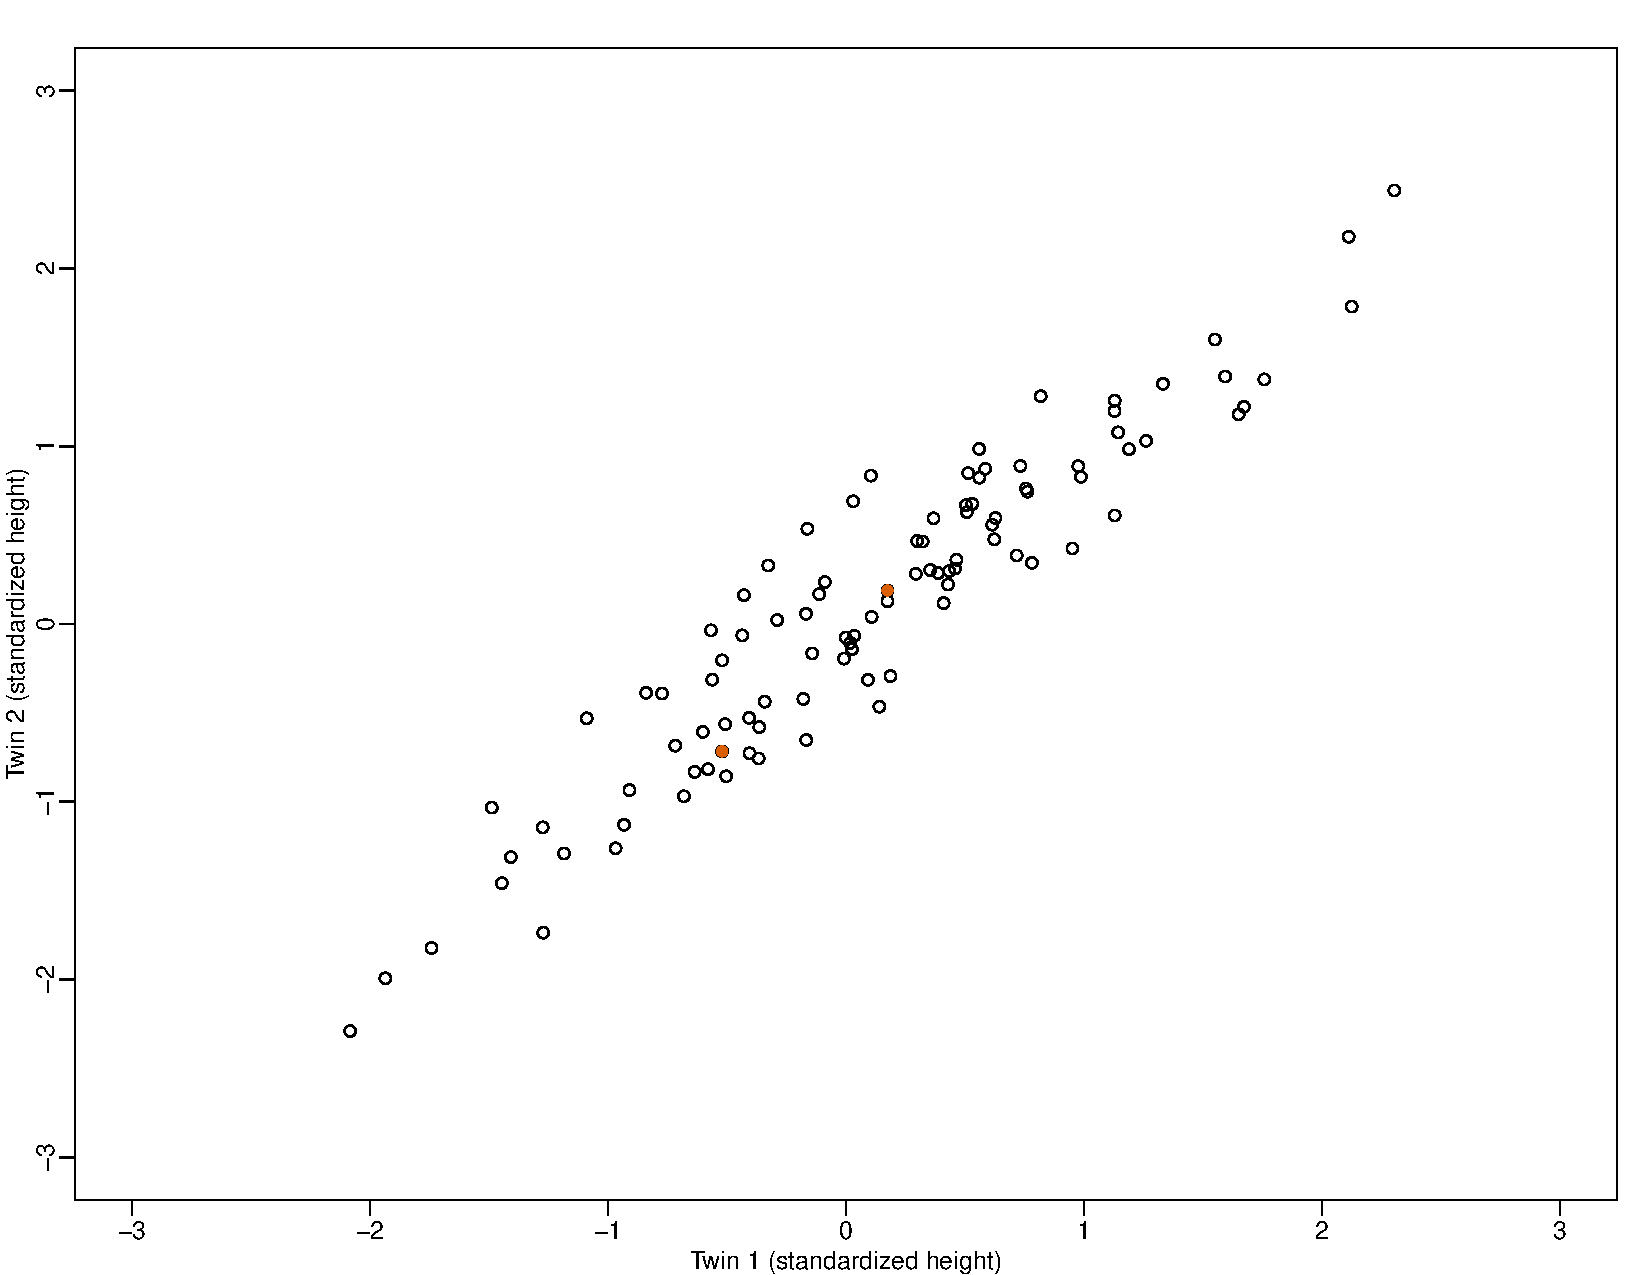
\includegraphics[width=1\textwidth,height=12.5in]{Firstplot.pdf}
\caption{Alt}
\end{figure}

You will notice that the data live in two dimensions, but they appear to
be somewhat linear. We can \emph{rotate} this plot so that it makes a
bit more sense, but taking the average of the twin heights and plotting
it against the difference of the heights. Let's take a look:

\begin{figure}
\centering
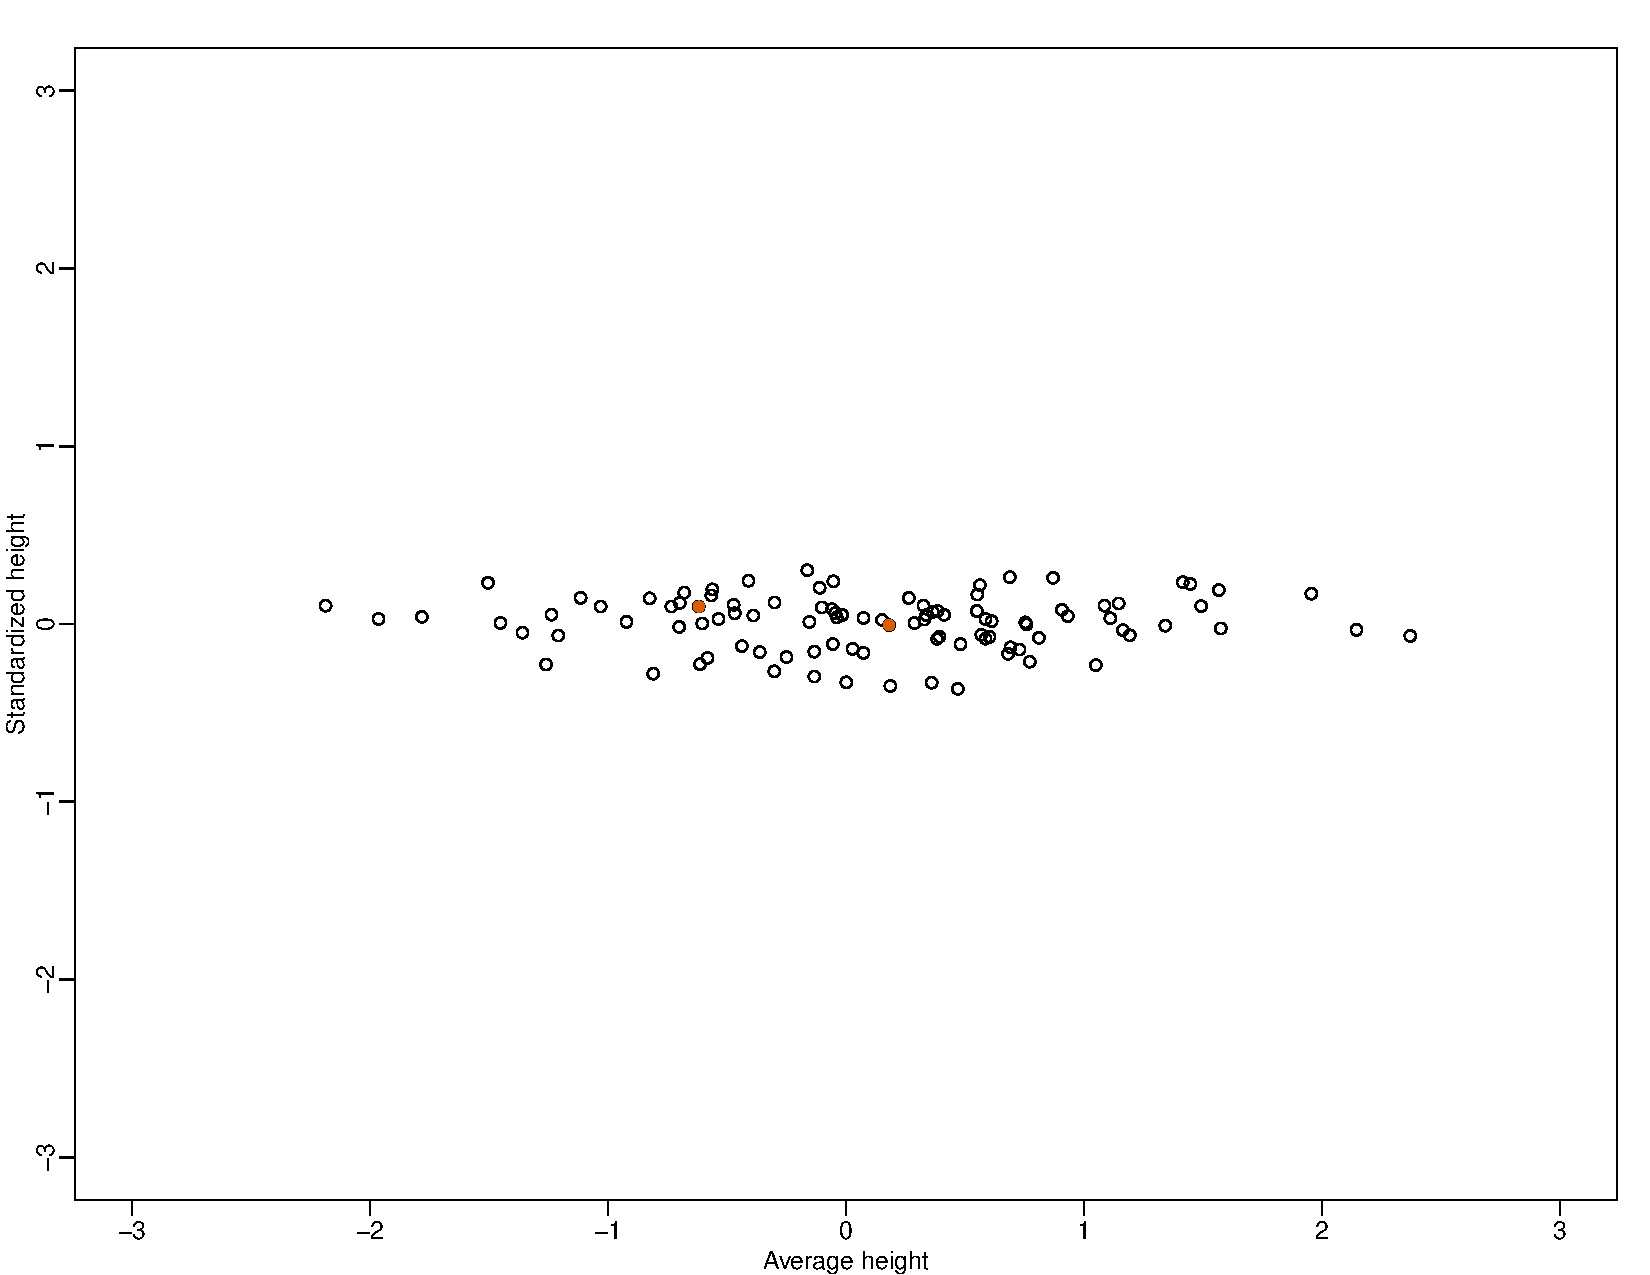
\includegraphics[width=1\textwidth,height=12.5in]{rotated.pdf}
\caption{Alt}
\end{figure}

The two orange points are the same in each plot, and you will note that
the rotation preserves the distance between them.

Now suppose you have expression levels for 1000 genes, and you want to
look at their plots. You can't visualize this in 1000 x 1000 space, and
if you do them pairwise you will need to examine almost 500,000 graphs.
This is just too much. Plus not all of the variables are, well,
interesting. So we want to reduce the dimensions.

One other thing to notice about the rotated graph: Most of the
``action'' is in the first dimension. This is the point, if you will, of
PCA. It allows us to summarize our data (our features, our variables)
with a smaller number of related variables that explain most of the
variability of our original data. That is, PCA gives you a
low-dimensional transformation of the data set such that these
components contain as much as possible of the variation. It gives you a
data representation in a smaller number of dimensions that are as
``interesting'''' as possible. By \emph{interesting} we mean here the
amount of variations of the observations in each dimension.

Just as we did with the example above, we seek a normalized, linear
combination of our features that has the highest variance, then the next
highest, etc.

Let's work through an example, continuing our work with the NCI60
dataset:

\begin{Shaded}
\begin{Highlighting}[]
\CommentTok{\# Find the principal components of the normalized data}
\NormalTok{pr.out }\OtherTok{\textless{}{-}} \FunctionTok{prcomp}\NormalTok{(nci.data, }\AttributeTok{scale =} \ConstantTok{TRUE}\NormalTok{)}

\CommentTok{\# Color assignment for each of the 64 cell lines}
\NormalTok{Cols }\OtherTok{\textless{}{-}} \ControlFlowTok{function}\NormalTok{(vec)\{}
\NormalTok{  cols}\OtherTok{=}\FunctionTok{rainbow}\NormalTok{(}\FunctionTok{length}\NormalTok{(}\FunctionTok{unique}\NormalTok{(vec)))}
  \FunctionTok{return}\NormalTok{(cols[}\FunctionTok{as.numeric}\NormalTok{(}\FunctionTok{as.factor}\NormalTok{(vec))])}
\NormalTok{\}}

\CommentTok{\# Plot the principal component score vectors}
\FunctionTok{par}\NormalTok{(}\AttributeTok{mfrow =} \FunctionTok{c}\NormalTok{(}\DecValTok{1}\NormalTok{, }\DecValTok{2}\NormalTok{), }\AttributeTok{pin =} \FunctionTok{c}\NormalTok{(}\DecValTok{3}\NormalTok{, }\DecValTok{3}\NormalTok{))}
\FunctionTok{plot}\NormalTok{(}
\NormalTok{  pr.out}\SpecialCharTok{$}\NormalTok{x[, }\DecValTok{1}\SpecialCharTok{:}\DecValTok{2}\NormalTok{],}
  \AttributeTok{col =} \FunctionTok{Cols}\NormalTok{(nci.labs),}
  \AttributeTok{pch =} \DecValTok{19}\NormalTok{,}
  \AttributeTok{xlab =} \StringTok{"Z1"}\NormalTok{,}
  \AttributeTok{ylab =} \StringTok{"Z2"}
\NormalTok{)}
\FunctionTok{plot}\NormalTok{(}
\NormalTok{  pr.out}\SpecialCharTok{$}\NormalTok{x[, }\FunctionTok{c}\NormalTok{(}\DecValTok{1}\NormalTok{, }\DecValTok{3}\NormalTok{)],}
  \AttributeTok{col =} \FunctionTok{Cols}\NormalTok{(nci.labs),}
  \AttributeTok{pch =} \DecValTok{19}\NormalTok{,}
  \AttributeTok{xlab =} \StringTok{"Z1"}\NormalTok{,}
  \AttributeTok{ylab =} \StringTok{"Z3"}
\NormalTok{)}
\end{Highlighting}
\end{Shaded}

\includegraphics{ML_part2_2021_files/figure-latex/unnamed-chunk-19-1.pdf}

These color plots aren't really all that interesting nor are they
particularly informative.

But wait, there's more!

Each component has a value associated with it that is the percent of
variance explained (PVE).

\begin{Shaded}
\begin{Highlighting}[]
\CommentTok{\# See what all is in the object}
\FunctionTok{summary}\NormalTok{(pr.out)}
\end{Highlighting}
\end{Shaded}

\begin{verbatim}
## Importance of components:
##                            PC1      PC2      PC3      PC4      PC5      PC6
## Standard deviation     27.8535 21.48136 19.82046 17.03256 15.97181 15.72108
## Proportion of Variance  0.1136  0.06756  0.05752  0.04248  0.03735  0.03619
## Cumulative Proportion   0.1136  0.18115  0.23867  0.28115  0.31850  0.35468
##                             PC7      PC8      PC9     PC10     PC11     PC12
## Standard deviation     14.47145 13.54427 13.14400 12.73860 12.68672 12.15769
## Proportion of Variance  0.03066  0.02686  0.02529  0.02376  0.02357  0.02164
## Cumulative Proportion   0.38534  0.41220  0.43750  0.46126  0.48482  0.50646
##                            PC13     PC14     PC15     PC16     PC17     PC18
## Standard deviation     11.83019 11.62554 11.43779 11.00051 10.65666 10.48880
## Proportion of Variance  0.02049  0.01979  0.01915  0.01772  0.01663  0.01611
## Cumulative Proportion   0.52695  0.54674  0.56590  0.58361  0.60024  0.61635
##                            PC19    PC20     PC21    PC22    PC23    PC24
## Standard deviation     10.43518 10.3219 10.14608 10.0544 9.90265 9.64766
## Proportion of Variance  0.01594  0.0156  0.01507  0.0148 0.01436 0.01363
## Cumulative Proportion   0.63229  0.6479  0.66296  0.6778 0.69212 0.70575
##                           PC25    PC26    PC27   PC28    PC29    PC30    PC31
## Standard deviation     9.50764 9.33253 9.27320 9.0900 8.98117 8.75003 8.59962
## Proportion of Variance 0.01324 0.01275 0.01259 0.0121 0.01181 0.01121 0.01083
## Cumulative Proportion  0.71899 0.73174 0.74433 0.7564 0.76824 0.77945 0.79027
##                           PC32    PC33    PC34    PC35    PC36    PC37    PC38
## Standard deviation     8.44738 8.37305 8.21579 8.15731 7.97465 7.90446 7.82127
## Proportion of Variance 0.01045 0.01026 0.00988 0.00974 0.00931 0.00915 0.00896
## Cumulative Proportion  0.80072 0.81099 0.82087 0.83061 0.83992 0.84907 0.85803
##                           PC39    PC40    PC41   PC42    PC43   PC44    PC45
## Standard deviation     7.72156 7.58603 7.45619 7.3444 7.10449 7.0131 6.95839
## Proportion of Variance 0.00873 0.00843 0.00814 0.0079 0.00739 0.0072 0.00709
## Cumulative Proportion  0.86676 0.87518 0.88332 0.8912 0.89861 0.9058 0.91290
##                          PC46    PC47    PC48    PC49    PC50    PC51    PC52
## Standard deviation     6.8663 6.80744 6.64763 6.61607 6.40793 6.21984 6.20326
## Proportion of Variance 0.0069 0.00678 0.00647 0.00641 0.00601 0.00566 0.00563
## Cumulative Proportion  0.9198 0.92659 0.93306 0.93947 0.94548 0.95114 0.95678
##                           PC53    PC54    PC55    PC56    PC57   PC58    PC59
## Standard deviation     6.06706 5.91805 5.91233 5.73539 5.47261 5.2921 5.02117
## Proportion of Variance 0.00539 0.00513 0.00512 0.00482 0.00438 0.0041 0.00369
## Cumulative Proportion  0.96216 0.96729 0.97241 0.97723 0.98161 0.9857 0.98940
##                           PC60    PC61    PC62    PC63      PC64
## Standard deviation     4.68398 4.17567 4.08212 4.04124 2.148e-14
## Proportion of Variance 0.00321 0.00255 0.00244 0.00239 0.000e+00
## Cumulative Proportion  0.99262 0.99517 0.99761 1.00000 1.000e+00
\end{verbatim}

\begin{Shaded}
\begin{Highlighting}[]
\FunctionTok{plot}\NormalTok{(pr.out)}
\end{Highlighting}
\end{Shaded}

\includegraphics{ML_part2_2021_files/figure-latex/unnamed-chunk-20-1.pdf}

\begin{Shaded}
\begin{Highlighting}[]
\NormalTok{pve }\OtherTok{=} \DecValTok{100} \SpecialCharTok{*}\NormalTok{ pr.out}\SpecialCharTok{$}\NormalTok{sdev }\SpecialCharTok{\^{}} \DecValTok{2} \SpecialCharTok{/} \FunctionTok{sum}\NormalTok{(pr.out}\SpecialCharTok{$}\NormalTok{sdev }\SpecialCharTok{\^{}} \DecValTok{2}\NormalTok{)}
\NormalTok{pve}
\end{Highlighting}
\end{Shaded}

\begin{verbatim}
##  [1] 1.135894e+01 6.756203e+00 5.751842e+00 4.247554e+00 3.734972e+00
##  [6] 3.618630e+00 3.066222e+00 2.685903e+00 2.529498e+00 2.375869e+00
## [11] 2.356558e+00 2.164122e+00 2.049097e+00 1.978818e+00 1.915417e+00
## [16] 1.771761e+00 1.662730e+00 1.610759e+00 1.594333e+00 1.559919e+00
## [21] 1.507217e+00 1.480099e+00 1.435762e+00 1.362771e+00 1.323502e+00
## [26] 1.275199e+00 1.259037e+00 1.209794e+00 1.180988e+00 1.120982e+00
## [31] 1.082774e+00 1.044775e+00 1.026471e+00 9.882745e-01 9.742571e-01
## [36] 9.311145e-01 9.147953e-01 8.956409e-01 8.729506e-01 8.425758e-01
## [41] 8.139798e-01 7.897498e-01 7.390010e-01 7.201016e-01 7.089184e-01
## [46] 6.902723e-01 6.784953e-01 6.470130e-01 6.408838e-01 6.011935e-01
## [51] 5.664186e-01 5.634028e-01 5.389352e-01 5.127863e-01 5.117962e-01
## [56] 4.816201e-01 4.384987e-01 4.100561e-01 3.691390e-01 3.212249e-01
## [61] 2.552891e-01 2.439782e-01 2.391163e-01 6.756902e-30
\end{verbatim}

\begin{Shaded}
\begin{Highlighting}[]
\FunctionTok{plot}\NormalTok{(}
\NormalTok{  pve,}
  \AttributeTok{type =} \StringTok{"o"}\NormalTok{,}
  \AttributeTok{ylab =} \StringTok{"Cumulative PVE"}\NormalTok{,}
  \AttributeTok{xlab =} \StringTok{"Principal Component"}\NormalTok{,}
  \AttributeTok{col =} \StringTok{"blue"}
\NormalTok{)}
\end{Highlighting}
\end{Shaded}

\includegraphics{ML_part2_2021_files/figure-latex/unnamed-chunk-20-2.pdf}

\begin{Shaded}
\begin{Highlighting}[]
\FunctionTok{plot}\NormalTok{(}
  \FunctionTok{cumsum}\NormalTok{(pve),}
  \AttributeTok{type =} \StringTok{"o"}\NormalTok{,}
  \AttributeTok{ylab =} \StringTok{"Cumulative PVE"}\NormalTok{,}
  \AttributeTok{xlab =} \StringTok{"Principal Component"}\NormalTok{,}
  \AttributeTok{col =} \StringTok{"brown3"}
\NormalTok{)}
\end{Highlighting}
\end{Shaded}

\includegraphics{ML_part2_2021_files/figure-latex/unnamed-chunk-20-3.pdf}

You will notice from the first plot that there is a drop-off (elbow) in
PVE from component 6 to 7. Also you will notice in the histogram that
there is a substantial dropoff in PVE going from component 1 to 2. So
you can safely reduce this dataset to representation by at most 6
components, and if you feel like living dangerously, to 2 components.
These are called scree plots. You should definitely look at these scree
plots as you evaluate the results of a principal components analysis,
and you should ask to see them as well for any that you happen upon in
your reading.

\hypertarget{multi-dimensional-scaling}{%
\subsubsection{Multi-dimensional
scaling}\label{multi-dimensional-scaling}}

Another unsupervised learning technique is Multi-dimensional Scaling
(MDS). We want to know about differences between observations. So, for
instance, let's consider the Khan dataset again. We are going to take
differences of the individual observations and the overall mean, then we
are going to use PCA again to examine the results. Except, since we are
doing this on the observation - mean differences, it is no longer
strictly PCA, and it is not called \emph{Principal Coordinate Analysis}
or PCoA. But the principles from PCA are still useful - we are going to
use the first two principal \emph{coordinates} to plot, because those
will capture most of the variability in these differences.

\begin{Shaded}
\begin{Highlighting}[]
\CommentTok{\# Use the nci.data set again}

\CommentTok{\# Assume we have N observations and p variables in an N x P dataset}

\FunctionTok{dim}\NormalTok{(nci.data)}
\end{Highlighting}
\end{Shaded}

\begin{verbatim}
## [1]   64 6830
\end{verbatim}

\begin{Shaded}
\begin{Highlighting}[]
\NormalTok{d }\OtherTok{\textless{}{-}} \FunctionTok{dist}\NormalTok{(nci.data)}
\NormalTok{fit }\OtherTok{\textless{}{-}} \FunctionTok{cmdscale}\NormalTok{(d, }\AttributeTok{eig=}\ConstantTok{TRUE}\NormalTok{, }\AttributeTok{k=}\DecValTok{2}\NormalTok{)}

\CommentTok{\# k is the number of principal coordinates we want}

\CommentTok{\# view the results}

\NormalTok{fit}
\end{Highlighting}
\end{Shaded}

\begin{verbatim}
## $points
##           [,1]        [,2]
## V1  -19.795782  -0.1152691
## V2  -21.546101   1.4573503
## V3  -25.056621  -1.5260929
## V4  -37.409536  11.3894784
## V5  -50.218642   1.3461737
## V6  -26.435203  -0.4629819
## V7  -27.339334  -2.6503128
## V8  -21.489658  -4.9541432
## V9  -20.852496 -10.1630615
## V10 -26.952915 -21.4733142
## V11 -24.446697  -9.8421205
## V12 -35.075028  -6.2621247
## V13 -21.483161 -10.6705481
## V14 -25.004732 -11.9464198
## V15 -31.745680 -14.9829235
## V16 -24.237312 -14.7479701
## V17 -20.503015 -16.1817793
## V18 -11.985682  -8.0623004
## V19 -24.344223  -3.7106407
## V20 -14.307441  -4.0257867
## V21 -11.696115 -11.5399627
## V22 -17.551264 -16.6589889
## V23 -10.158885   1.5009404
## V24   2.609693  -7.0693601
## V25   4.273638 -14.7401698
## V26  -7.003487 -14.7512986
## V27   2.175539 -10.0689995
## V28 -10.390669 -17.2133665
## V29  -4.105585 -12.8336713
## V30  -3.107199 -13.5041785
## V31 -13.920131 -10.7706320
## V32  -7.340931 -11.8634764
## V33  -5.031984  -1.6785213
## V34  21.303920   6.0889181
## V35  38.922020   3.6351811
## V36  46.441061   4.8194665
## V37  48.513831   7.0614137
## V38  41.878712   6.9915000
## V39  56.922686   9.5122363
## V40  50.959323   8.1773536
## V41  26.031599   8.7690748
## V42  11.818059  -8.0595882
## V43  31.654807  -6.5893268
## V44  26.333583 -15.0839917
## V45  20.568131 -18.2511162
## V46  21.536202 -13.4346199
## V47  34.669827 -13.2857448
## V48  18.605803 -17.0724922
## V49  38.194352 -13.3673940
## V50  38.155371 -11.5925449
## V51  30.893122 -12.9394271
## V52  21.585841  -9.8917234
## V53   3.110738 -17.6582405
## V54   9.160494  -1.4605448
## V55  14.878915  -0.6309639
## V56   5.272994  45.4663832
## V57  -3.319772  46.3001255
## V58   1.321339  51.3627117
## V59 -11.087277  37.6788847
## V60 -15.446086  44.1646074
## V61  -1.925437  35.3286112
## V62 -14.359566  33.2916782
## V63 -12.740136  45.2228727
## V64  -8.377818  34.2231717
## 
## $eig
##  [1]  3.989258e+04  2.223445e+04  1.763489e+04  1.153423e+04  1.030411e+04
##  [6]  9.393097e+03  7.704158e+03  7.546846e+03  7.067195e+03  5.777779e+03
## [11]  5.625239e+03  5.363188e+03  4.903092e+03  4.734148e+03  4.479053e+03
## [16]  4.313525e+03  4.226112e+03  3.894810e+03  3.877879e+03  3.781525e+03
## [21]  3.678888e+03  3.463529e+03  3.376313e+03  3.171466e+03  3.159457e+03
## [26]  2.971593e+03  2.843771e+03  2.760077e+03  2.721835e+03  2.662913e+03
## [31]  2.567680e+03  2.513886e+03  2.346339e+03  2.321256e+03  2.241116e+03
## [36]  2.217796e+03  2.172898e+03  2.140319e+03  2.031981e+03  1.998809e+03
## [41]  1.955073e+03  1.914526e+03  1.875043e+03  1.823102e+03  1.784005e+03
## [46]  1.686705e+03  1.667479e+03  1.586297e+03  1.466288e+03  1.438720e+03
## [51]  1.386747e+03  1.312147e+03  1.270309e+03  1.226021e+03  1.150863e+03
## [56]  1.118501e+03  1.051878e+03  9.678660e+02  9.040303e+02  7.823942e+02
## [61]  6.567918e+02  6.262224e+02  5.615703e+02 -1.445337e-12
## 
## $x
## NULL
## 
## $ac
## [1] 0
## 
## $GOF
## [1] 0.2319364 0.2319364
\end{verbatim}

\begin{Shaded}
\begin{Highlighting}[]
\CommentTok{\# plot it}

\NormalTok{x }\OtherTok{\textless{}{-}}\NormalTok{ fit}\SpecialCharTok{$}\NormalTok{points[,}\DecValTok{1}\NormalTok{]}
\NormalTok{y }\OtherTok{\textless{}{-}}\NormalTok{ fit}\SpecialCharTok{$}\NormalTok{points[,}\DecValTok{2}\NormalTok{]}

\FunctionTok{plot}\NormalTok{(x, y, }\AttributeTok{xlab =} \StringTok{"PCo1"}\NormalTok{, }\AttributeTok{ylab =} \StringTok{"PCo2"}\NormalTok{,}
     \AttributeTok{main =} \StringTok{"Metric MDS"}\NormalTok{, }\AttributeTok{type =} \StringTok{"n"}\NormalTok{)}
\FunctionTok{text}\NormalTok{(x, y, }\AttributeTok{labels =}\NormalTok{ nci.labs, }\AttributeTok{cex =} \FloatTok{0.7}\NormalTok{)}
\end{Highlighting}
\end{Shaded}

\includegraphics{ML_part2_2021_files/figure-latex/unnamed-chunk-21-1.pdf}

We can also do what is called nonmetric MDS, using a function from the
MASS package.

\begin{Shaded}
\begin{Highlighting}[]
\FunctionTok{library}\NormalTok{(MASS)}

\NormalTok{fit }\OtherTok{\textless{}{-}} \FunctionTok{isoMDS}\NormalTok{(d, }\AttributeTok{k=}\DecValTok{2}\NormalTok{)}
\end{Highlighting}
\end{Shaded}

\begin{verbatim}
## initial  value 30.903164 
## iter   5 value 20.778162
## iter   5 value 20.760297
## iter   5 value 20.750556
## final  value 20.750556 
## converged
\end{verbatim}

\begin{Shaded}
\begin{Highlighting}[]
\NormalTok{x }\OtherTok{\textless{}{-}}\NormalTok{ fit}\SpecialCharTok{$}\NormalTok{points[,}\DecValTok{1}\NormalTok{]}
\NormalTok{y }\OtherTok{\textless{}{-}}\NormalTok{ fit}\SpecialCharTok{$}\NormalTok{points[,}\DecValTok{2}\NormalTok{]}

\FunctionTok{plot}\NormalTok{(x, y, }\AttributeTok{xlab =} \StringTok{"PCo1"}\NormalTok{, }\AttributeTok{ylab =} \StringTok{"PCo2"}\NormalTok{,}
     \AttributeTok{main =} \StringTok{"nonMetric MDS"}\NormalTok{, }\AttributeTok{type =} \StringTok{"n"}\NormalTok{)}
\FunctionTok{text}\NormalTok{(x, y, }\AttributeTok{labels =}\NormalTok{ nci.labs, }\AttributeTok{cex =} \FloatTok{0.7}\NormalTok{)}
\end{Highlighting}
\end{Shaded}

\includegraphics{ML_part2_2021_files/figure-latex/unnamed-chunk-22-1.pdf}

\end{document}
